%% Hello emacs, this is -*- latex -*-
\typeout{ ====================================================================}
\typeout{ This is file msc.tex, created at 03-Jun-2004 }
\typeout{ Maintained by Andre Rabello dos Anjos <Andre.dos.Anjos@cern.ch> }
\typeout{ ====================================================================}

\chapter{Processamento de Dados de Calorimetria}
\label{chap:msc}

Redes Neurais Artificiais (RNA's) vêm sendo utilizadas em muitos experimentos
em Física de Altas Energias \cite{nnet-hera, daq11, nnet-hep, nnet-cdf}. Neste
capítulo apresenta-se uma técnica para empregar RNA's no Segundo Nível de
Filtragem do experimento ATLAS, especificamente para o problema da
discriminação elétron/jato, usando dados dos calorímetros deste detetor. A
confirmação da ocorrência de elétrons é de suma importância para o
experimento \cite{trigger-tpr}.

\section{A Cadeia de Processamento no LVL2}

Quando o Primeiro Nível de Filtragem (LVL1) deteta a ocorrência de objetos
interessantes nos calorímetros, o Segundo Nível de Filtragem deve começar seu
processamento confirmando esta decisão. Para isso, poderá requisitar aos ROS's
dados para todas as camadas do calorímetro do ATLAS ao redor da RoI
destacada. Entre os objetos que podem interessar ao LVL1 estão RoI's que
indicam a ocorrência de elétrons ou fótons altamente energéticos no evento. O
LVL1 não consegue, devido a sua baixa granularidade de informação, distinguir
elétrons de fótons e então chama estes objetos genericamente de
``eletromagnéticos'' ou e.m..

E\-lé\-trons e fó\-tons, por sua vez, representam canais muito comuns no
experimento~\cite{trigger-tpr}. Estes elementos, no entanto, sofrem
freqüentemente a contaminação por jatos de partículas bastante colimadas, que
podem interagir com os calorímetros imitando assinaturas e.m.. Estes jatos
colimados confundem o LVL1, pois têm características de deposição e isolamento
muito semelhantes a de elétrons e fótons, novamente levando-se em consideração
a granularidade de processamento no LVL1. Uma análise mais apurada somente
poderá ser conduzida no LVL2.

No LVL2, três atividades são conduzidas durante a discriminação de objetos
e.m.:

\begin{enumerate}
\item Preparação dos dados: nesta primeira etapa, os dados carregados dos
ROS's são desempacotados e preparados para a fase de extração de
características que sucede. Durante o processamento, os dados são convertidos
para um formato mais apropriado para a discriminação e calibrados de acordo
com constantes disponibilizadas durante a configuração da L2PU;

\item Extração de características: esta fase do processamento calcula o valor
de quantidades-padrão para a discriminação de objetos e.m.. Uma descrição
completa destas variáveis é destacada a seguir;

\item Discriminação: é a última fase do processamento, onde o sistema de
filtragem cria uma hipótese sobre um objeto baseando-se nas quantidades
calculadas. No caso de objetos e.m., as hipóteses podem ser: elétrons, fótons
ou não-e.m., este último indicando que o objeto foi equivocadamente
classificado como e.m. pelo LVL1, causando a rejeição do evento por completo.
\end{enumerate}

%% Observação: seria interessante ter um ou dois parágrafos aqui do que vai
%% mostrado. Seixas, 28-junho-2004.

\section{O espaço de entrada para os discriminadores de objetos e.m.}
\label{sec:datainput}

Objetos e.m. são analisados normalmente em uma região $0,4\times0,4$ no plano
$\eta\times\phi$. Isto compreende uma área de $4\times4$ torres de filtragem
para os calorímetros e.m. do ATLAS e de $2\times2$ torres de filtragem para os
calorímetros hadrônicos.

Devido à granularidade variante de cada camada com $\eta$ e de camada para
camada nos calorímetros do ATLAS, o número de células total para uma RoI do
calorímetro pode variar bastante. Além disso, como mostram as
Tabelas~\ref{tab:lar} e \ref{tab:had}, há regiões nas quais algumas camadas
não estão presentes. Por exemplo, o \eng{presampler} somente existe até
$\eta=1,8$. Este tipo de situação deve ser tratada, de forma a se compor um
vetor de entrada compatível com o sistema de classificação que atuará na fase
final do processamento.

A Figura~\ref{fig:ncell} mostra o número médio de células por RoI, extraído de
alguns arquivos contendo dados de elétrons e jatos que interagem com os
calorímetros do ATLAS. As barras de erro representam a falta de estatística ao
longo de $\phi$\footnote{A curva foi traçada criando-se um histograma
bi-dimensional ao longo das direções $\eta$ e $\phi$, e depositando em cada
caixa (\eng{bin}), o número médio de células de todas as RoI que tinham seu
centro naquele canal. As diversas curvas ao longo de $\phi$ foram somadas e
produziram uma média (linha cheia) e um desvio padrão (barras de erro) para
cada um de seus pontos em $\eta$.} . No eixo das abscissas é possível ver os
valores de $\eta$, e no eixo das coordenadas, o número de células na seção
e.m., hadrônica e total (somando-se o número de células nas duas seções).

\begin{figure}
\begin{center}
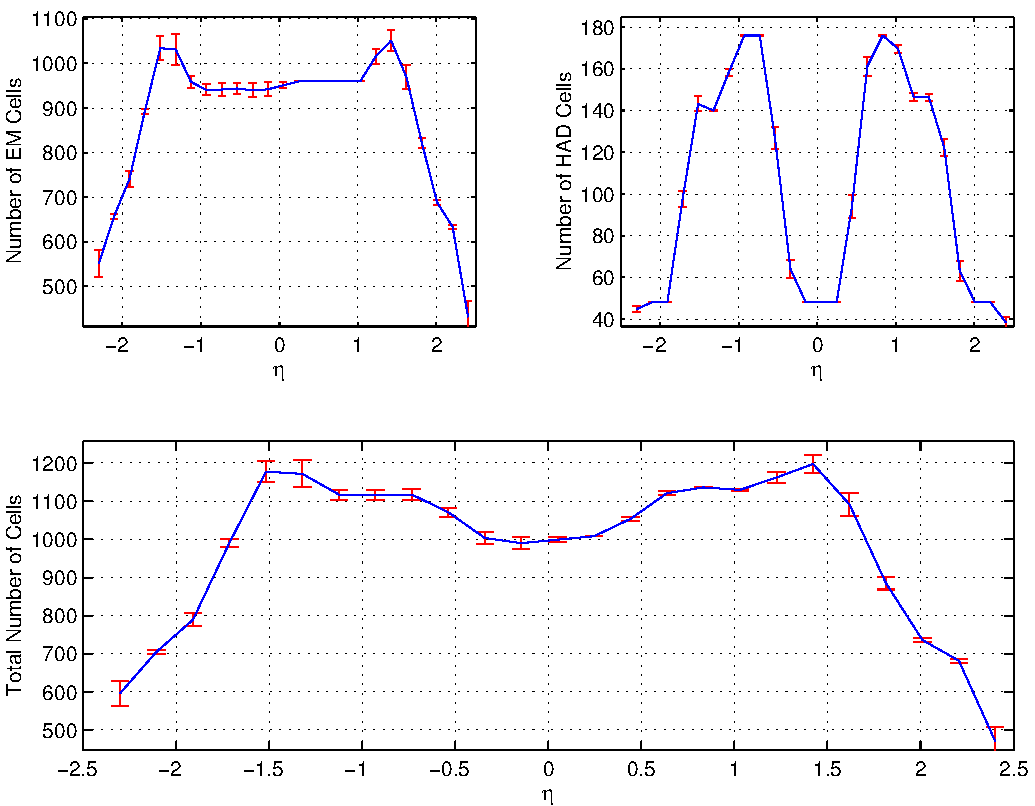
\includegraphics[scale=0.65]{msc/all-granularity}
\end{center}
\caption[O número médio de células por RoI's de diversos objetos e.m..]{O número
médio de células por RoI's de diversos objetos e.m.. A parte superior do
gráfico representa o número de células nas seções e.m. e hadrônica dos
calorímetros, da esquerda para a direita. Na parte inferior é possível ver o
total de células nas duas seções.}
\label{fig:ncell}
\end{figure}

O contorno dos gráficos é coerente, considerando-se as Tabelas~\ref{tab:lar} e
\ref{tab:had}. O número de células da RoI, na seção hadrônica, é a que mais
varia. Os picos, começando em $|\eta|=0,8$ e se estendendo até $|\eta|=1,0$,
representam o início do barril estendido e o final do barril (TileCal). Na
região central ($\eta=0$), o número de células é $4\times4\times3=48$, pois há
3 camadas, cada uma com 16 células, como mostra a Tabela~\ref{tab:had}. O
número de células nas laterais da figura cai vertiginosamente. O pico, situado
aproximadamente em $|\eta|=1,5$, representa o início da tampa, que também
perde granularidade rapidamente com o aumento de $|\eta|$.

O número de células na seção e.m. varia menos que o equivalente na seção
hadrônica. Há uma constância no número de células até aproximadamente
$|\eta|=1,3$, quando a tampa começa, mostrando um pico que culmina em
$|\eta|=1,475$, ou seja, no início da terceira camada na tampa. Após
$|\eta|=1,5$, o número de células cai vertiginosamente com o aumento do módulo
da pseudo-rapidez, até $|\eta|=2,5$, quando a tampa acaba.

Existem algumas soluções para o problema de granularidade variante de RoI para
RoI. Esta proposta, no entanto, limita o seu escopo na investigação de uma
abordagem com \emph{Vários pré-processadores, um único discriminador}. Esta
abordagem determina a construção de um número de pré-processadores e
extratores de características que são acionados conforme a localidade da RoI
investigada. O número de quantidades calculadas é constante, independente do
módulo de pré-processamento ativado. Este enfoque facilita a implementação do
sistema de discriminação. Ademais, como será visto mais à frente, cortes de
dimensionalidade nos dados de entrada podem tornar o pré-processamento
genérico o suficiente para atender um grande número de possibilidades, sem
perdas significativas no desempenho de classificação.

Inicialmente, trabalhar-se-á somente com RoI's para os quais o centro possui
valores de $|\eta_{\text{centro}}|<1,3$. Desta forma, não se tem que lidar com
problemas mais complicados de granularidade e é possível focalizar os estudos
no método em si. Mais tarde será visto que é possível reduzir estas restrições
facilmente, considerando-se a relevância dos dados de entrada. Ademais, para
reduzir-se a dimensão de entrada, as células do \eng{plug} conectado ao barril
estendido são somadas às células correspondentes naquele detetor. As células
de regiões onde há uma sobreposição entre o barril e sua extensão também são
somadas. A Figura~\ref{fig:eroi} mostra uma RoI de um elétron típico,
interagindo com as diversas camadas do calorímetro. As somas propostas acima
já foram efetuadas. Cada bloco representa a energia depositada naquela
célula. Na parte superior desta figura, é possível ver o \eng{presampler}
seguindo-se das 3 camadas eletromagnéticas e das 3 camadas hadrônicas. Como é
possível ver, um elétron desenvolve sua cascata de forma bem concentrada, ao
redor do ponto de impacto. Da terceira camada e.m. em diante, não há
praticamente informação relevante, predominando o ruído, já que o objeto perde
energia rapidamente devido à forma específica com que interage com o volume do
detetor.

\begin{figure}
\begin{center}
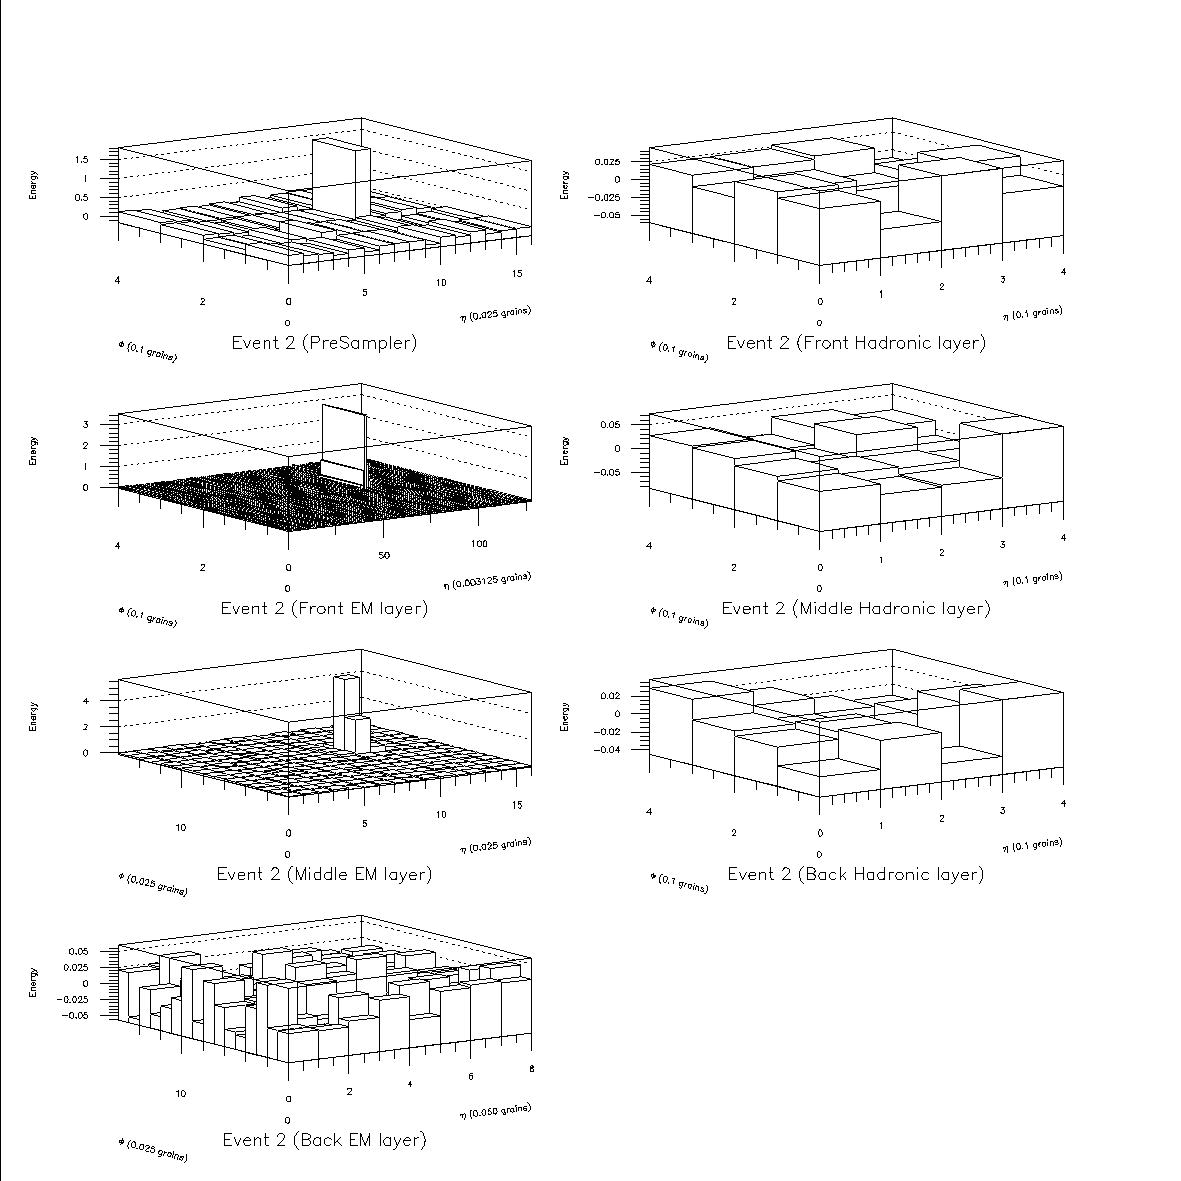
\includegraphics[scale=0.6]{msc/typical-electron}
\end{center}
\caption{Uma RoI de um elétron típico interagindo com o calorímetro.}
\label{fig:eroi}
\end{figure}

A Figura~\ref{fig:jroi}, por sua vez, mostra uma RoI típica de um jato. Repare
que a deposição de energia no calorímetro hadrônico torna este objeto bastante
óbvio para qualquer classificador. A Figura~\ref{fig:ejet} mostra, no entanto,
um jato bem mais difícil de ser corretamente classificado pois sua cascata
possui um padrão de deposição que o faz muito parecido com um elétron. Devido
à discriminação realizada no LVL1, os eventos (jatos) que falsearam o disparo
do sistema para elétrons, tendem a ser predominantemente deste tipo, tornando
a classificação correta dos eventos uma tarefa desafiadora. Somente um
discriminador que explore muito bem as nuances no perfil de deposição de
objetos e.m. conseguirá classificá-lo corretamente.

\begin{figure}
\begin{center}
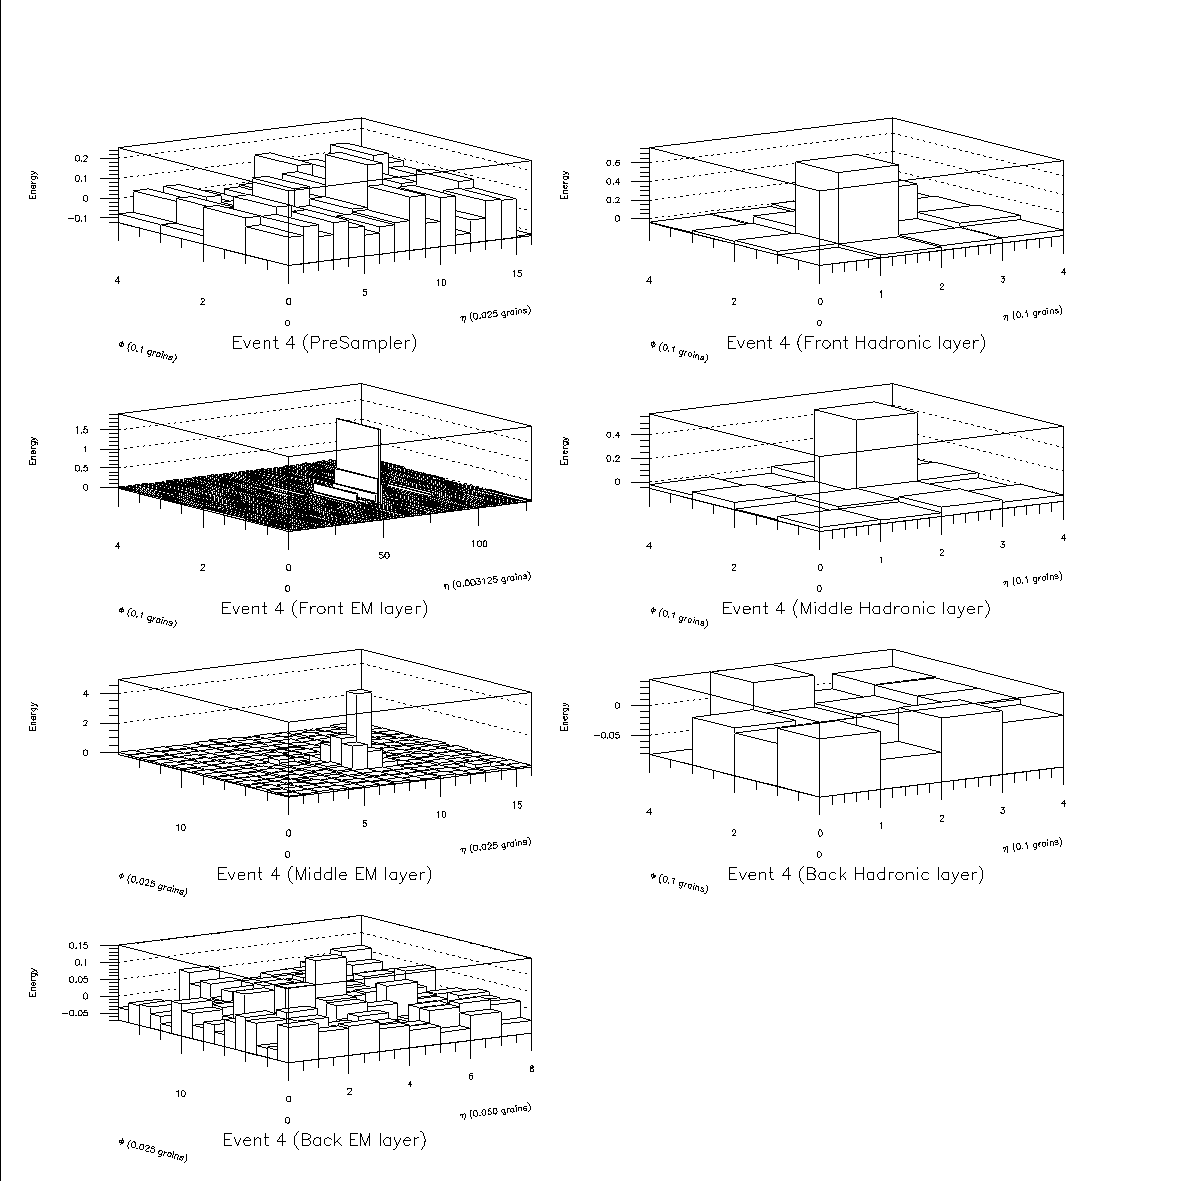
\includegraphics[scale=0.7]{msc/typical-jet}
\end{center}
\caption{Uma RoI de um jato típico interagindo com o calorímetro.}
\label{fig:jroi}
\end{figure}

\begin{figure}
\begin{center}
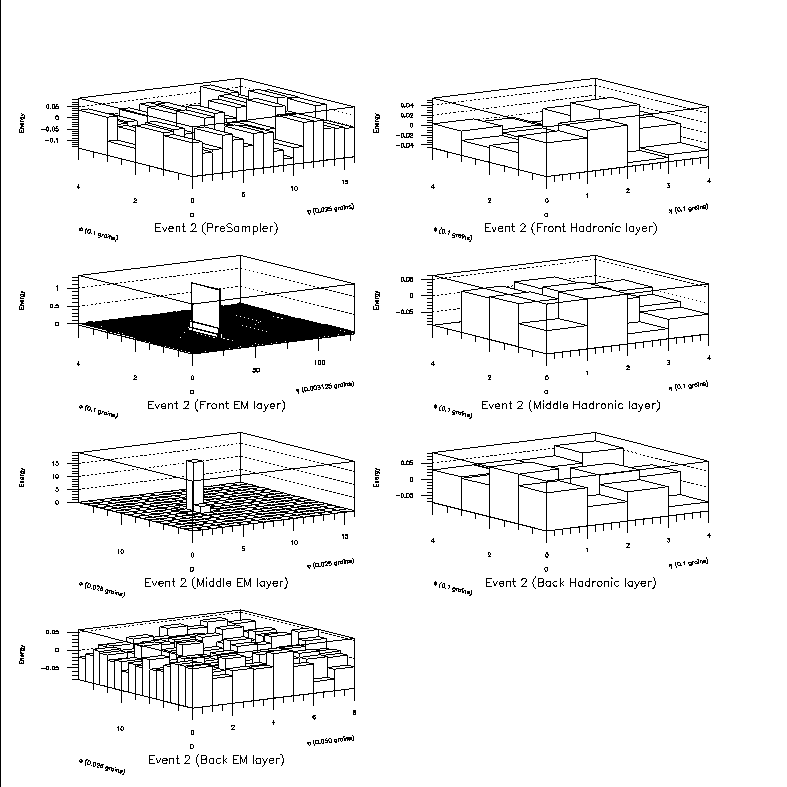
\includegraphics[scale=0.7]{msc/ejet}
\end{center}
\caption{Uma RoI de um jato cujos padrões de deposição de energia fazem-no
parecer um elétron interagindo com o calorímetro.}
\label{fig:ejet}
\end{figure}

\subsubsection{A terceira camada e.m.}

A 3\eira\ camada e.m. possui uma granularidade que varia bastante com
$\eta$. Para evitar maiores complicações durante a implementação dos
discriminadores neste trabalho, eliminar-se-á a informação desta camada no
processo. Espera-se que o sistema consiga, através de correlações de ordens
mais elevadas, recuperar esta informação. Isto também representará uma redução
significativa no tempo de processamento da RoI, já que os dados desta camada
não serão movidos para o processador local ou processados pelo sistema.

\section{Os dados disponíveis}
\label{sec:inputdata}

Considerando todos os eventos disponíveis, dispõe-se de cerca de 600 RoIs de
elétrons e cerca de 3600 de jatos. A seguir, discutem-se algumas das
características do dados disponíveis:

\begin{description}
\item[Energia Transversa] Os elétrons têm energia transversa aproximadamente
igual a 20 GeV. A energia transversa para o conjunto de jatos varia, pois a
técnica de discriminação empregada no L1 não leva em consideração a energia
depositada nos calorímetros hadrônicos, onde este tipo de objeto interage mais
intensamente, depositando a maior parte de sua energia.

Objetos e.m. com baixa energia (ou seja, na faixa de dezenas de GeV) são mais
difíceis de serem classificados \cite{hlt-tdr}. Por isto, testes com
discriminadores são realizados prioritariamente com elementos nessa faixa
energética.

\item[Empilhamento] Por causa da taxa elevada de eventos, o detetor ATLAS
sofrerá efeitos de empilhamento (do inglês, \eng{pile-up}). Empilhamento é o
efeito causado nos detetores devido a sobreposição de eventos (um evento que
ainda se desenvolve no detetor tem seu padrão de deposição de energia
distorcido por um novo evento que chega e se sobrepõe ao evento). Ele gera um
\textit{pedestal}, ou seja, um ruído muito forte, aos eventos sendo
analisados. Os dados disponíveis não têm a simulação deste efeito. Alguns
estudos \cite{seixas:pileup, seixas:perf-loss}, no entanto, sugerem que haja
uma perda de aproximadamente 2\% no desempenho de discriminação, ao adicionar
o efeito pedestal aos eventos, quando se utiliza de processamento neuronal para
as RoI's.
\end{description}

\section{O Processamento clássico de objetos e.m.}
\label{sec:classical}

A colaboração ATRIG (\eng{ATLAS Trigger}) desenvolveu um algoritmo para
realizar a separa\-ção e\-lé\-tron\-/\-jato nas condições do LHC, comumente
chamado de \textsf{T2Calo}. Este algoritmo é baseado no conhecimento
especialista de físicos experimentais. Ele extrai quatro quantidades físicas,
que são altamente discriminantes. Neste caso, a extração de características
será ainda feita à parte. Chamar-se-ão estas quatro quantidades de
\emph{quantidades clássicas} no decorrer do texto.

As quatro variáveis extraídas para a discriminação se encontram descritas a
seguir. Como é possível ver, são, na maior parte, derivadas de somas
energéticas, o que é implementável de forma extremamente veloz.

\begin{description}
\item[\etem] Esta quantidade representa a soma das energias das células da
seção e.m. dos calorímetros, cujo centro recai sobre uma região de
0,075$\times$0,175 no plano \ep, ao redor do centro da célula da segunda camada
e.m. que apresenta o maior valor de energia depositada. A janela é irregular
por motivos da física de interesse \cite{hlt-tdr}. A região na qual esta
quantidade é extraída equivale, usando-se a granularidade da segunda camada
e.m., a uma região de 3 células na direção $\eta$ por 7 células na direção de
$\phi$. Espera-se que a energia de elétrons esteja totalmente contida nesta
janela; por seu turno, jatos devem apresentar, hipoteticamente, uma fração
menor de sua energia depositada nesta área;

\item[\ethad] Esta quantidade representa a soma das células da seção hadrônica
do calorímetro dentro de uma região de 0,2$\times$0,2 no plano \ep, ao redor
do centro da célula na segunda camada e.m. que apresenta o maior valor de
energia depositada. Para elétrons, a quantidade de energia depositada na
camada hadrônica deve ser próxima de zero, enquanto que, para jatos, espera-se
que seja bem elevada;

\item[\rshape] Representa a razão entre a soma das células na segunda camada
e.m., numa área de $3\times7$ células por $7\times7$ células ao redor da célula
na segunda camada que apresenta o maior valor de energia depositado. Esta
quantidade mede o espalhamento da cascata formada pelo decaimento do objeto de
estudo. No caso do objeto ser um jato, espera-se que a cascata tenha um
espalhamento maior que no caso de elétrons, resultando em um valor menor que 1
para esta quantidade;

\item[\rstrip] Uma vez que jatos de par\-tí\-culas interagem de forma mais
espalhada do que e\-lé\-trons, espera-se que na primeira camada e.m. sejam
observados vários picos. Definindo um pico ($E$) como sendo a ocorrência de um
máximo registrado pela célula central de um agrupamento de três células
adjacentes, então, a quantidade \rstrip\ representa a razão de energias
\rstrip$=\frac{E_1-E_2}{E_1+E_2}$. Ou seja, a razão da subtração pela soma dos
valores de energia dos dois picos mais energéticos na primeira camada e.m..

Se o objeto for um elétron (objeto único), espera-se que $E_2=0$, já que a
cascata de partículas que o elétron forma na sua interação com o calorímetro é,
tipicamente, bastante estreita, e portanto \rstrip=1. Para jatos, normalmente,
\rstrip será menor que 1, já que $E_2\neq0$.
\end{description}

\subsection{Eficiência de discriminação}
\label{sec:eff-classical}

Implementou-se um sistema de pré-processamento que extrai as quantidades
descritas acima dos arquivos de dados. Nas Figuras~\ref{fig:dados-2d} e
\ref{fig:dados-3d}, é possível ver projeções bi e tri-dimensionais destas 4
variáveis. É possível notar que algumas variáveis possuem uma variância
pequena para elétrons e grande para jatos. A partir destas quantidades,
desenvolveram-se alguns discriminadores para avaliar o desempenho da
formulação clássica na separação elétron/jato.

\begin{figure}
\begin{center}
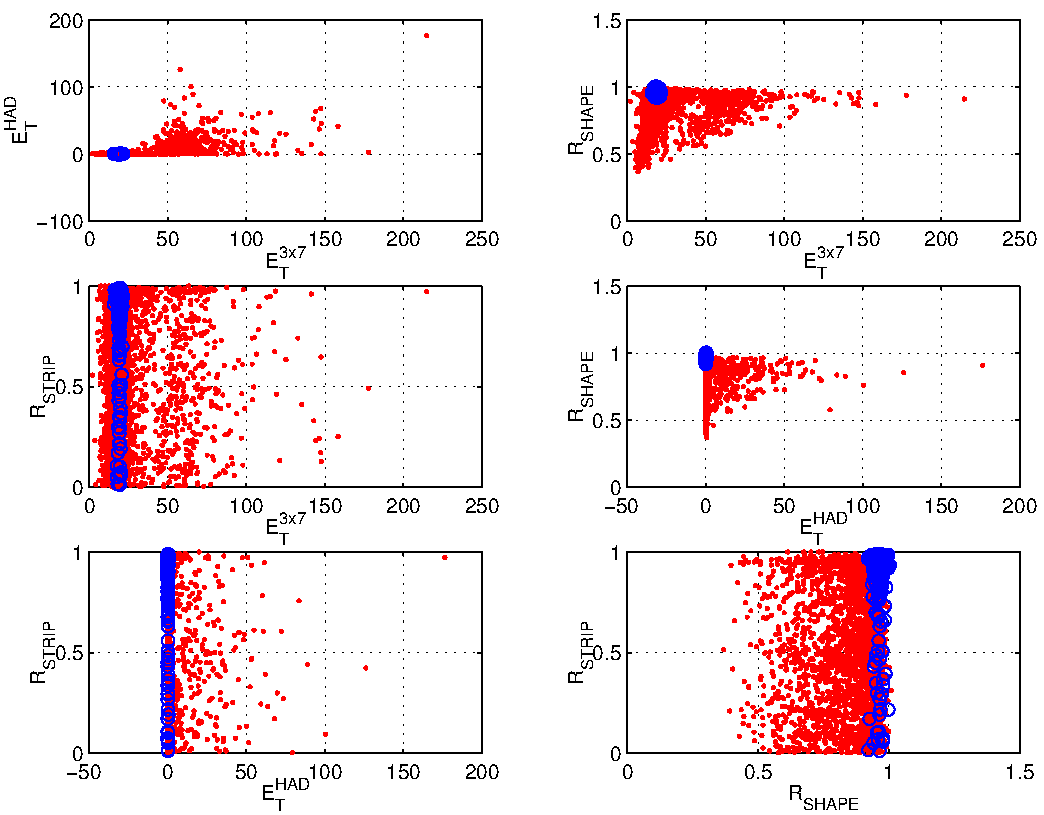
\includegraphics[scale=0.65]{msc/view2d}
\end{center}
\caption[Variáveis clássicas em planos bi-dimensionais.]{Variáveis clássicas em
planos bi-dimensionais. Elétrons estão representados por círculos azuis
enquanto jatos, por pontos vermelhos.}
\label{fig:dados-2d}
\end{figure}

\begin{figure}
\begin{center}
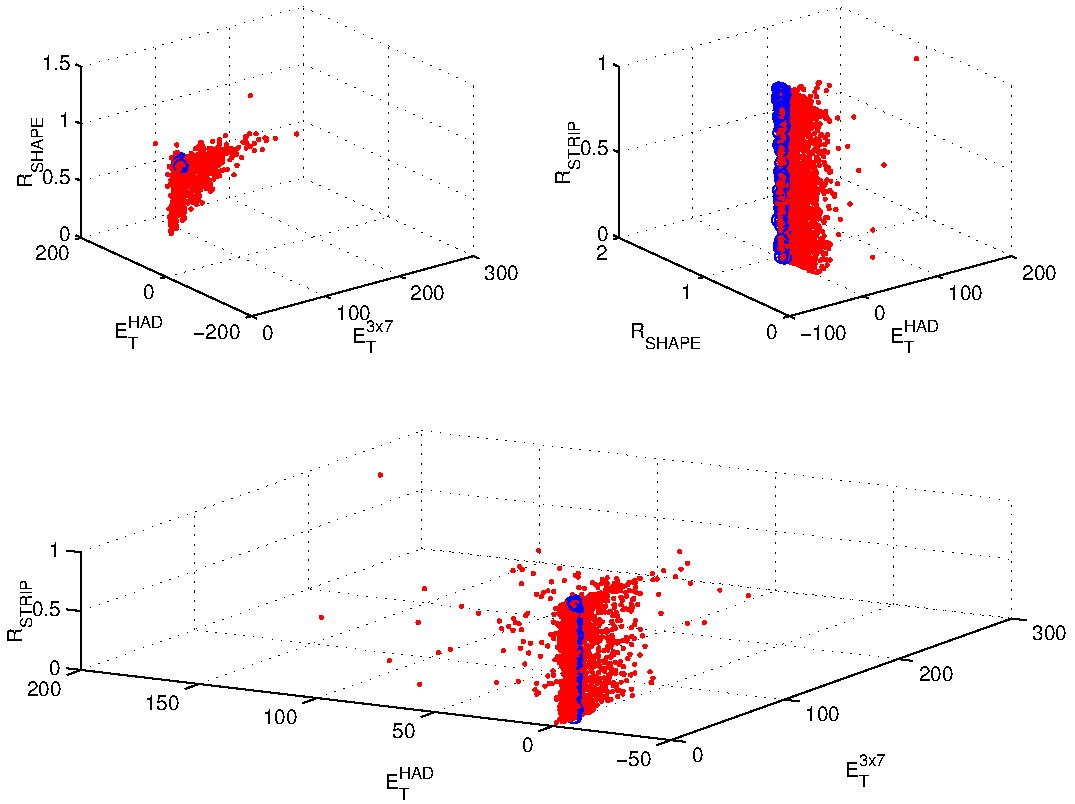
\includegraphics[scale=0.65]{msc/view3d}
\end{center}
\caption[Variáveis clássicas em planos tri-dimensionais.]{Variáveis clássicas
em planos tri-dimensionais. Elétrons estão representados por círculos azuis
enquanto jatos, por pontos vermelhos.}
\label{fig:dados-3d}
\end{figure}

Os testes foram feitos utilizando-se cerca de 270 elétrons e 3600 jatos
(separados em duas metades, uma para treino e outra para teste), que estavam
disponíveis nos arquivos de dados\footnote{Os dados são obtidos através de
simulações de Monte Carlo, utilizando a configuração atual de detetores e as
técnicas de filtragem de eventos do ATLAS. Por esta razão, o número de
elétrons gerados (provenientes de decaimentos de bósons de Higgs) é bastante
menor que o número de jatos, já que a ocorrência de um Higgs é um processo
raro.}. Os elétrons utilizados nestes testes são um sub-conjunto dos 600
elétrons que foram mencionados na Seção~\ref{sec:inputdata}. Os jatos são
exatamente os mesmos. A razão de ter se reduzido o conjunto de dados repousa
no fato que o algoritmo necessita da maior granularidade disponível para
maximizar sua eficiência de discriminação e os 330 elétrons restantes não
possuem a informação da terceira camada bem definida.

O projeto dos discriminadores é conduzido utilizando-se metade dos dois
conjuntos de dados, ou seja, 135 elétrons e 1800 jatos. O segundo conjunto de
dados somente é usado para testar os discriminadores encontrados.

A seguir, se enumeram e se detalham alguns possíveis discriminadores baseados
nestas quatro quantidades físicas.

\subsection{Discriminador Linear}

Nesta modalidade, calcula-se o hiper-plano no espaço das 4 variáveis que
melhor discrimina elétrons e jatos, utilizando o algoritmo LMS (\eng{Least
Mean Squares}, ou método dos mínimos quadrados iterativo). Utilizando um
neurônio linear, o mínimo global está bem-definido no espaço proposto pelas 4
variáveis e é alcançado facilmente com a escolha correta da taxa de
aprendizado \cite{widrow, haykin}.

Esta solução não explora bem situações nas quais o domínio das variáveis de
uma das classes está dentro do domínio das variáveis da outra classe (como é
possível ver nos gráficos das Figuras~\ref{fig:dados-2d} e
\ref{fig:dados-3d}). Dois ou mais patamares de separação por dimensão, neste
caso, seriam mais apropriados. Por esta razão, este discriminador não produz
resultados tão bons como na separação através da análise combinatória das
variáveis duas a duas, conforme é feito pelos físicos especialistas, ou
separadores neuronais, que podem esboçar recortes mais sofisticados no
subespaço formado por estas quatro variáveis.

O discriminador, em si, consiste apenas de um neurônio, cuja função de
ativação é a identidade (neurônio \textit{linear}). Os valores iniciais de
pesos para a entrada e para a polarização (\eng{bias}) são escolhidos
aleatoriamente, durante a inicialização do treinamento. Os alvos ($t_i$) para
as classes de elétrons e jatos são, respectivamente, $+1$ e $-1$. O sistema é
treinado em bateladas de 100 eventos (usando-se o algoritmo LMS), até que o
erro médio quadrático das saídas ($o_i$) da rede, calculado sobre
\textbf{todos} os ($N$) vetores de entrada disponíveis (EMQ,
Equação~\ref{eq:emq}), se estabilize. Para isto, o conjunto de treinamento é
divido nas classes elétron e jato e 50 eventos de cada classe, escolhidos
aleatoriamente, são apresentados à rede para que se dê um passo de
treinamento.

\begin{equation}
\text{EMQ} = \frac{1}{N} \sum^N_{i=1}(t_i-o_i)^2
\label{eq:emq}
\end{equation}

Após 30.000 passos de treinamento, o erro médio quadrático para o conjunto de
treinamento estabilizou-se em 0,63 e para o conjunto de teste em 0,67. O
resultado se repetiu para diferentes inicializações (o teste foi realizado 3
vezes). A Figura~\ref{fig:mse-linear} mostra a evolução do erro médio
quadrático para os conjuntos de teste e treinamento. Nessa figura, é possível ver
que o sistema converge de forma suave para o valor de EMQ final.

\begin{figure}
\begin{center}
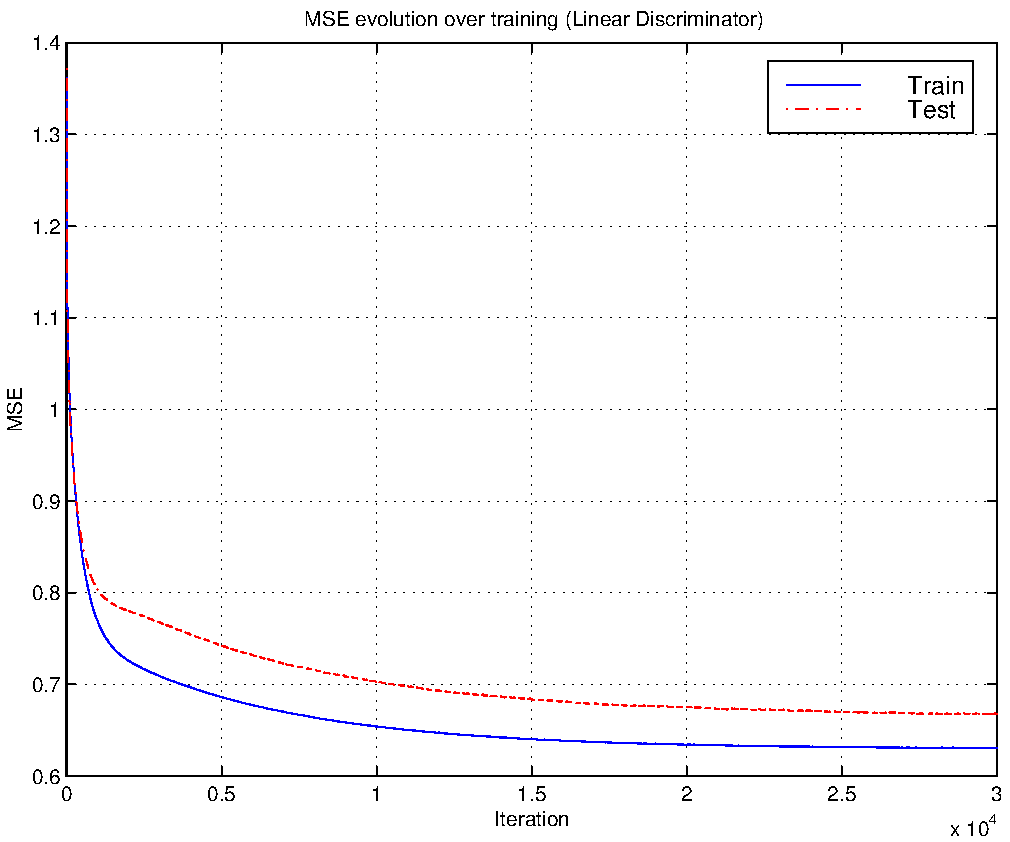
\includegraphics[scale=0.6]{msc/mselinear}
\end{center}
\caption{A evolução do EMQ para o discriminador linear}
\label{fig:mse-linear}
\end{figure}

À saída do discriminador linear (agora treinado), aplica-se um patamar de
separação (\eng{threshold}). Objetos cujas saídas estão à esquerda do patamar,
são considerados como jatos, todos os outros, como elétrons. Cada patamar que
é proposto implica num valor de eficiência de discriminação para ambas as
classes que estão sendo separadas, formando a curva característica do detetor
(ROC, do inglês, \eng{Receiver Operation Characteristics})
\cite{vantrees}. Patamares mais à esquerda (aproximando-se de $-1$)
privilegiarão elétrons, não só aumentando a probabilidade de deteção do sinal
de interesse, mas também a probabilidade de falso alarme, enquanto que mais à
direita (aproximando-se de $+1$), jatos são privilegiados, não somente
reduzindo o falso alarme, mas também a probabilidade de deteção (de elétrons).

É possível determinar um conjunto de coordenadas que representem a eficiência
de discriminação de elétrons e jatos, à medida que desloca-se o patamar de
separação, da esquerda para a direita. Analogamente, a este conjunto de
coordenadas, existe outro que representa a eficiência de discriminação em
elétrons contra o erro na classifição de jatos. A Figura~\ref{fig:linear}
mostra a curva de eficiência obtida considerando-se os diferentes patamares de
separação. Neste caso, os valores no eixo das abscissas foram multiplicados
por 25 (kHz)\footnote{Este número é extraído de \cite{daqnote00-02}. Ele
representa a taxa de objetos que são erroneamente classificados como elétrons
pelo L1 e, portanto, a taxa de elétrons ``falsos" que o L2 receberá.}, pois
há, de fato, interesse na eficiência de classificação de elétrons, contra a
taxa de falso alarme real (i.e., do sistema de filtragem) em jatos, ou seja, o
número de jatos erroneamente classificados como elétrons (vide
equação~\ref{eq:noise}). Portanto, por exemplo, para 86\% de eficiência em
elétrons, a eficência para jatos é 28,2\%.

\begin{figure}
\begin{center}
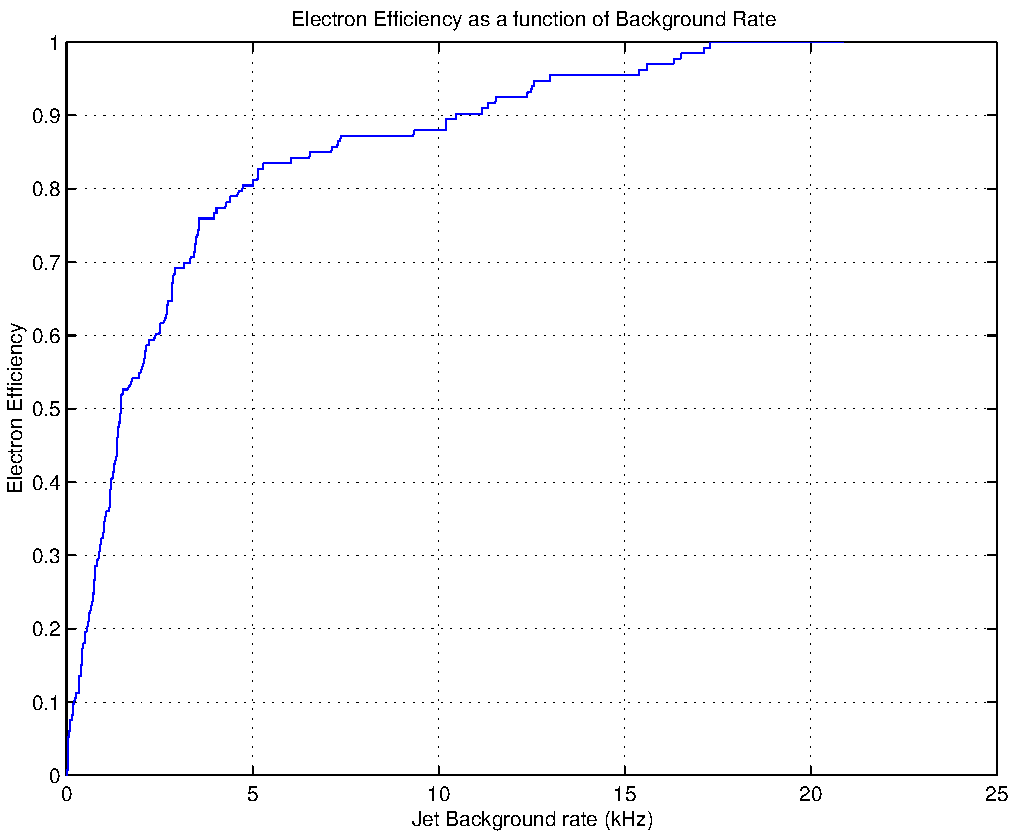
\includegraphics[scale=0.5]{msc/lineareff}
\end{center}
\caption[A curva de eficiência para um separador linear ótimo aplicado às 4
variáveis físicas descritas.]{A curva de eficiência para um separador linear
ótimo aplicado às 4 variáveis físicas descritas. No eixo das coordenadas
encontra-se a eficiência no acerto de elétrons, enquanto que no eixo das
coordenadas, a taxa de ruído (jatos erroneamente classificados), em kHz.}
\label{fig:linear}
\end{figure}

\begin{equation}
\text{Falso Alarme Real} = 25 \text{kHz} \times (1 - \text{Eficiência para
jatos})
\label{eq:noise}
\end{equation}

\subsection{Discriminador por Análise Combinatória}

Neste caso, estudam-se as correla\-çõ\-es entre as va\-ri\-á\-ve\-is duas a
duas, determinando um separador linear por plano de análise. O processo
continua até que todas as permutações tenham sido analisadas. É o método
atualmente utilizado no CERN e classicamente usado pelos físicos, como forma
de superar as dificuldades em se analisar o comportamenteo das variáveis de
discriminação em espaços de dimensionalidade elevada, onde a visualização
completa do comportamento discriminante dessas variáveis não é
possível. Espera-se que o resultado aqui seja um pouco melhor do que no caso
anterior, pois este enfoque explora o conhecimento da física do
evento. Ademais, esta técnica permite que um conjunto de recortes mais
sofisticados seja aplicado, de forma a classificar melhor as duas classes de
objetos.

É claro que a ordem na qual se averiguam os 6 espaços bi-dimensionais é
extremamente relevante para um desempenho satisfatório do discriminador, já
que não é possível anteceder acuradamente que alguns eventos poderão ser
separados de forma mais eficaz pelos próximos níveis de separação. O
projetista deve ter um bom conhecimento das variáveis e suas distribuições
para operar desta forma. Para a referência do leitor, realizou-se o exercício
de discriminação analisando as combinações de variáveis duas a duas segundo à
ordem descrita na Tabela~\ref{tab:config}. A primeira dessas configurações é a
ordem mais intuitiva de separação de objetos e.m., baseando-se nas descrições
das variáveis e sua relevância em \cite{daqnote00-02, hlt-tdr}. A segunda
configuração é a primeira com sua ordem invertida e com a 3\eira\ e 4\eira\
etapas trocadas.

\newcommand{\vez}{$\times$}
\begin{table}
\caption{Configurações para um pos\-sí\-vel discriminador por a\-ná\-lise
combina\-tó\-ria das variáveis duas a duas (\textit{clás\-sico}).}
\label{tab:config}
\begin{center}
\begin{tabular}{|c|l|l|} \hline
Etapa & Configuração 1 & Configuração 2 \\ \hline
1     & \etem\vez\ethad    & \rstrip\vez\rshape \\
2     & \etem\vez\rshape   & \rstrip\vez\ethad \\
3     & \etem\vez\rstrip   & \rstrip\vez\etem \\
4     & \ethad\vez\rshape  & \rshape\vez\ethad \\
5     & \ethad\vez\rstrip  & \rshape\vez\etem \\
6     & \rshape\vez\rstrip & \ethad\vez\etem \\ \hline
\end{tabular}
\end{center}
\end{table}

Para construir os 6 separadores lineares, utiliza-se do sistema mostrado na
figura~\ref{fig:bidim-scheme}. Na parte inferior dessa figura é possível
averiguar que o sistema de filtragem nesse caso estará configurado em
cascata. Cada etapa de filtragem eliminará mais jatos, tentando reter o maior
número de elétrons possível. A parte superior da figura mostra o funcionamento
de cada bloco da cascata. Esses blocos são compostos de um sistema de entrada
gráfica e um algoritmo de treinamento usando LMS.

\begin{figure}
\begin{center}
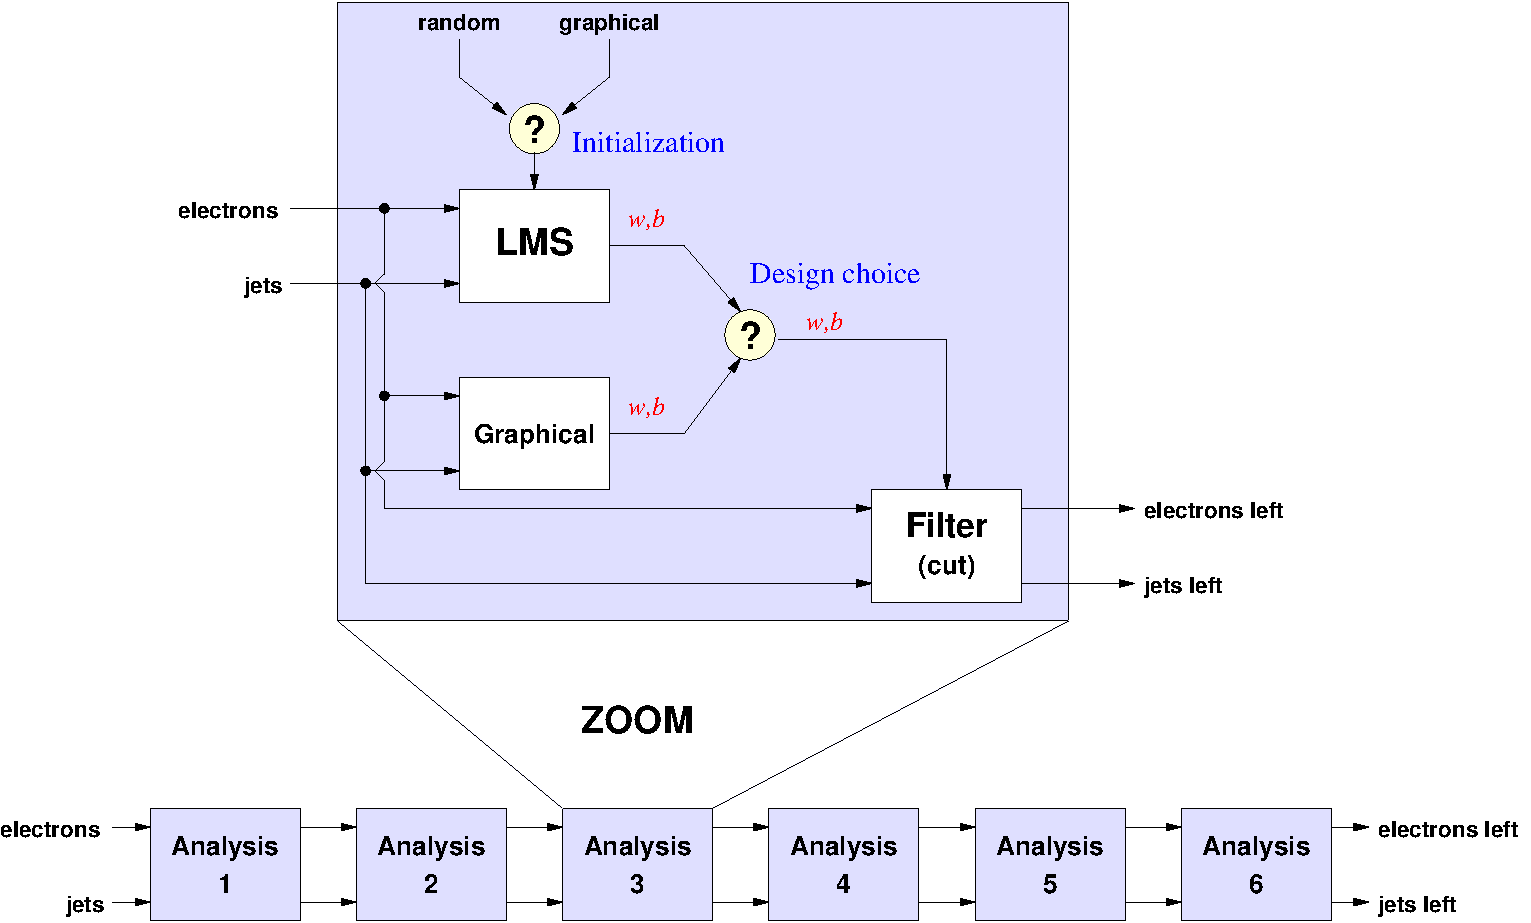
\includegraphics[scale=0.55]{msc/bidim-scheme}
\end{center}
\caption[O esquema que determina o separador por análise combinatória das 4
variáveis clássicas quando agrupadas em pares.]{O esquema que determina o
separador por análise combinatória das 4 variáveis clássicas quando agrupadas
em pares (veja texto).}
\label{fig:bidim-scheme}
\end{figure}

O projeto de cada bloco inicia-se escolhendo a polarização e os pesos através
de um sistema gráfico ou de forma aleatória. Os eventos de entrada são
divididos em conjuntos de treinamento e teste e são normalizados\footnote{As
variáveis \etem e \ethad tiveram as médias de classe removidas e foram
divididas pelo desvio padrão da respectiva distribuição. As demais (\rstrip e
\rshape) não sofreram alterações, pois se encontravam contidas no intervalo entre
0 e 1, não sendo necessário uma normalização adicional.}. Os valores iniciais
de peso e polarização então, são utilizados para a inicialização do algoritmo
de treinamento, que calcula o plano separador com o menor EMQ possível usando
como entrada para rede as duas variáveis escolhidas para a etapa de treinamento
atual. O treinamento é parado quando os valores de EMQ para os conjuntos de
teste e treino atingem seus mínimos ou quando o EMQ se mostra com uma variação
muito menor (10000 vezes) que sua amplitude entre dois passos de treinamento
consecutivos. Utilizou-se o treinamento em bateladas de 10 eventos.

Após minimizar o EMQ, o sistema desenhará no plano escolhido os vetores
relativos a cada objeto sob análise e confirma para o projetista o plano de
separação. Nesse momento, o projetista poderá alterar o plano graficamente, se
assim desejar, invalidando a minimização pelo EMQ. Independente do escolhido,
um separador será utilizado por um filtro linear, já na saída do bloco, para
discriminar os objetos na entrada do sistema. À saída do filtro, um patamar de
separação em 0 (zero) é aplicado: eventos cujas saídas são maiores ou iguais a
zero são resguardados, enquanto que os demais são descartados. Os eventos
remanescentes são utilizados para um processo análogo de projeto da próxima
etapa de filtragem.

\subsubsection{Resultados}
\label{sec:bi-results}

A curva de eficiência deste separador é difícil de ser traçada, já que deve-se
sintonizar 6 retas ao invés de um único plano no caso linear! Com algum
esforço seria possível esboçar alguns pontos no plano eficiência
\eng{versus} falso alarme; pontos esses que representam projeções da superfície
no hiper-plano de dimensão 6 que realmente define a curva de eficiência deste
discriminador. Já que este trabalho foge do escopo deste projeto, limita-se a
descrever as eficiências de separação elétron/jato para os dois casos
descritos, com o patamar de separação afixado em 0 para todos os 6
discriminadores lineares:

\begin{enumerate}
\item Configuração 1 - Conseguiu-se, ao final, que 95\% dos elétrons fossem
corretamente classificados enquanto que apenas 2,91 kHz de jatos fossem
admitidos (88,4\% de eficiência na deteção de jatos);
\item Configuração 2 - Neste caso termina-se o processo com 93\% de eficiência
de elétrons contra apenas 3,58 kHz (85,7\% de eficiência) de taxa de jatos
(jatos).
\end{enumerate}

Para o caso linear, a mesma eficiência de deteção de elétrons implica em uma
taxa de jatos de 12,9 kHz (48,3\% de eficiência) e 12,2 kHz (51,3\% de
eficiência) respectivamente para as configurações 1 e 2. Esses resultados são
obtidos a partir da curva na Figura~\ref{fig:linear}, e confirmam a melhoria
obtida com a nova técnica.

\subsection{Discriminador Neuronal}

Neste caso, treinou-se uma rede neuronal sem realimentação e totalmente
conectada, com 4 neurônios não-lineares (com função de ativação tipo
\emph{tangente hiperbólica}) na camada intermediária \cite{haykin}, para que
se faça a separação entre elétrons e jatos. Os dados de entrada foram
normalizados da mesma forma que na seção anterior, de tal forma que não mais
que 10\% dos eventos se encontrassem fora do intervalo ${-1,+1}$.

A rede foi treinada em bateladas, usando-se o método de retro-propagação dos
erros, com taxa de aprendizado variável e momento \cite{haykin, hertz}
usando-se o pacote JETNET, versão 3.0 \cite{jetnet}. As
equações~\ref{eq:momentum} e \ref{eq:decay} descrevem a utilização do momento
($\mu$) e do decaimento no aprendizado ($\gamma$) da rede,
respectivamente. Nestas equações $E$ representa o erro médio quadrático (EMQ)
e a matriz $\boldsymbol{w}$ o valor dos pesos da rede \cite{jetnet}. Na
equação~\ref{eq:momentum} é possível ver que valores muito altos de momento
(próximos à unidade) podem trazer instabilidade ao sistema, já que o valor
efetivo da atualização dos pesos sinápticos torna-se muito alto \cite{hertz}.

\begin{equation}
\Delta \boldsymbol{w}_{t+1} = -\mu\frac{\partial E}{\partial \boldsymbol{w}_{t+1}} + \alpha\cdot\Delta \boldsymbol{w}_{t}
\label{eq:momentum}
\end{equation}

\begin{equation}
\mu_{t+1} = 
\begin{cases}
\mu_{t}\cdot\gamma& \text{se } E_{t+1} > E_t \\
\mu_{t}\cdot\bigl(1+\frac{1-\gamma}{10}\bigr)& \text{caso contrário}
\end{cases}
\label{eq:decay}
\end{equation}

\subsubsection{Resultados}

Um total de 23 redes foram treinadas com parâmetros de taxa de aprendizado
($\mu$), momento ($\alpha$) e decaimento ($\gamma$) diferentes. A
inicialização dos pesos foi feita de forma aleatória para cada teste,
escolhendo-se um número real entre $-1$ e $+1$. O critério de parada utilizado
é o produto SP, que será explanado em detalhes mais a frente
(Seção~\ref{sec:sp}). Basicamente, o produto SP é a soma das eficiências de
discriminação de elétrons e jatos multiplicado pelo produto das
mesmas. Utilizar o erro médio quadrático para este fim, neste caso, não é
conveniente, pois se está interessado na eficiência de discriminação da rede
\cite{haykin}.

A Tabela~\ref{tab:class-neural} mostra os resultados obtidos após o
treinamento dessas várias redes. A primeira coluna mostra o número do
teste. As colunas seguintes indicam, respectivamente, a taxa de aprendizado, o
momento, a taxa de decaimento da taxa de aprendizado, o valor do produto SP, o
número total de passos de treinamento, o tamanho da batelada, o número da
iteração onde o melhor produto SP foi obtido, o erro médio quadrático ao final
do treinamento, o patamar de separação entre as classes (que garante o produto
SP ótimo apresentado), as eficiências de discriminação para elétrons e jatos
naquele patamar e o ruído de fundo (jatos) resultante do erro de discriminação
de jatos. Os resultados (valores de eficiência e EMQ) são representativos do
conjunto de teste, ou seja, aquele que \textbf{não} foi utilizado para treinar
a rede neuronal. O tamanho da época para todos os casos foi mantido fixo em
100 (passos de treinamento).

Durante esses testes, verificaram-se as seguintes propriedades do sistema:

\begin{itemize}
\item Tamanho da batelada e taxa de aprendizado - Utilizando uma taxa de
aprendizado alta, a rede tende a obter resultados melhores (maior produto
SP). Como conseqüência, há maior oscilação nos valores de EMQ durante o
treinamento, o que pode ser reduzido optando-se por um treinamento mais longo
usando uma taxa de aprendizado bem menor (em torno de 0,01) ou aumentando o
tamanho da batelada e inserindo um amortecimento à taxa de aprendizado
($\gamma$). Utilizaram-se bateladas com diferentes tamanhos (100, 400, 600,
800 e 1000). Dentre estas opções, a rede que apresentou convergência mais
suave, tinha sua batelada igual a 1000;

\item Suscetibilidade ao momento - Ao adicionar à atualização dos pesos a
informação do passo anterior, através do momento ($\mu$), o sistema apresenta
um forte comportamento oscilatório. Valores de momento acima de 0,9 são
suficientes para que o fenômeno ocorra, o que já era esperado \cite{hertz};

\item Produto SP e o EMQ - Analisando a Tabela~\ref{tab:class-neural}, é
possível ver que o EMQ não tem, de fato, total correlação com o valor do
produto SP. Na grande maioria dos testes, o valor do produto SP foi acima de
1,5, chegando a um valor máximo de 1,57 em alguns casos. Já o valor do EMQ,
para os mesmos testes, variou bastante, havendo casos onde dobrava, embora o
desempenho de discriminação da rede permanecesse constante;

\item Patamar de separação - O patamar de separação\footnote{O melhor patamar
de separação representa o ponto no intervalo $[-1,+1]$ que gera o maior
produto SP.} está, na grande maioria das vezes, à direita do zero, indicando
que as redes treinadas conseguem identificar bem elétrons, mas não são tão
eficazes na idenficação de jatos. Este resultado era esperado, pois os jatos
que chegam ao segundo nível são de difícil classificação e apresentam uma
flutuação estatística maior que o sinal de elétrons, bem mais estável. O fato
do patamar estar muitas vezes à direita do zero também pode indicar que a
classe de elétrons tem um EMQ menor que a de jatos;

\end{itemize}

% The result table
\renewcommand{\baselinestretch}{1}
\begin{table}
\caption{Os resultados do treinamento de 23 redes neurais para
separação elétron/jato utilizando as quatro variáveis clássicas.}
\label{tab:class-neural}
\renewcommand{\baselinestretch}{1.25}
\small
\begin{center}
\begin{sideways}
\begin{tabular}{|c|c|c|c|c|c|c|c|c|c|c|c|c|} \hline
Teste & $\mu$ & $\alpha$ & $\gamma$ & SP & \# Passos & \# Batelada & Itera��o &
EMQ & Patamar & \% e$^-$ & \% jatos & Falso alarme (kHz) \\ \hline\hline

1 & 0,15 & 0,5 & 1 & 1,55 & 1000 & 100 & 954 & 0,368 & 0,243 & 95 &
89,07 & 2,73 \\ \hline

2 & 0,15 & 0,7 & 1 & 1,57 & 1000 & 100 & 900 & 0,572 & 0,715 & 94 &
90,45 & 2,39 \\ \hline

3 & 0,15 & 0,9 & 1 & 1,57 & 1000 & 100 & 757 & 0,311 & 0,039 & 96 &
88,96 & 2,76 \\ \hline

4 & 0,15 & 0,99 & 1 & 1,54 & 1000 & 100 & 149 & 0,210 & -0,696 & 96 &
88,02 & 2,99 \\ \hline

5 & 0,05 & 0,9 & 1 & 1,57 & 1000 & 100 & 726 & 0,452 & 0,550 & 93 &
91,39 & 2,15 \\ \hline

6 & 0,02 & 0,9 & 1 & 1,54 & 1000 & 100 & 953 & 0,419 & 0,281 & 95 &
88,63 & 2,84 \\ \hline

7 & 0,02 & 0,95 & 1 & 1,57 & 1500 & 100 & 1366 & 0,287 & 0,148 & 93 &
91,11 & 2,22 \\ \hline

8 & 0,02 & 0,995 & 1 & 1,55 & 1500 & 100 & 348 & 0,411 & 0,559 & 93 &
90,34 & 2,41 \\ \hline

9 & 0,01 & 0,95 & 1 & 1,56 & 2000 & 100 & 1845 & 0,300 & 0,133 & 94 &
90,07 & 2,48 \\ \hline

10 & 0,09 & 0,75 & 1 & 1,56 & 1000 & 400 & 706 & 0,344 & 0,125 & 96 &
87,80 & 3,05 \\ \hline

11 & 0,07 & 0,75 & 1 & 1,55 & 1000 & 400 & 925 & 0,319 & 0,069 & 96 &
87,75 & 3,06 \\ \hline

12 & 0,1 & 0,75 & 1 & 1,55 & 1000 & 600 & 616 & 0,345 & 0,128 & 96 &
87,75 & 3,06 \\ \hline

13 & 0,1 & 0,75 & 1 & 1,56 & 1000 & 1000 & 573 & 0,330 & 0,067 & 96 &
87,80 & 3,05 \\ \hline

14 & 0,1 & 0 & 1 & 1,47 & 1000 & 1000 & 791 & 0,493 & 0,195 & 94 &
86,53 & 3,37 \\ \hline

15 & 0,15 & 0 & 1 & 1,52 & 1000 & 1000 & 787 & 0,290 & 0,418 & 92 &
90,73 & 2,32 \\ \hline

16 & 0,15 & 0 & 1 & 1,53 & 1000 & 800 & 886 & 0,378 & 0,466 & 93 &
90,34 & 2,41 \\ \hline

17 & 0,15 & 0 & 0,95 & 1,53 & 1000 & 800 & 941 & 0,548 & 0,491 & 93 &
90,34 & 2,41 \\ \hline

18 & 0,15 & 0 & 0,9 & 1,53 & 1000 & 800 & 946 & 0,578 & 0,528 & 93 &
90,45 & 2,39 \\ \hline

19 & 0,1 & 0 & 0,7 & 1,51 & 1500 & 600 & 999 & 0,412 & 0,262 & 93 &
89,79 & 2,55 \\ \hline

20 & 0,15 & 0,75 & 0,7 & 1,56 & 1300 & 600 & 757 & 0,250 & -0,083 & 95 &
89,24 & 2,69 \\ \hline 

21 & 0,15 & 0,9 & 0,7 & 1,56 & 1300 & 600 & 360 & 0,301 & 0,098 & 95 &
89,29 & 2,68 \\ \hline

22 & 0,15 & 0,5 & 0,6 & 1,55 & 1300 & 600 & 1179 & 0,363 & 0,164 & 96 &
87,69 & 3,08 \\ \hline

23 & 0,05 & 0,75 & 0,7 & 1,55 & 2500 & 800 & 2190 & 0,283 & 0,115 & 93 &
90,62 & 2,35 \\ \hline 
\end{tabular}

\end{sideways}
\end{center}
\end{table}
\renewcommand{\baselinestretch}{1.5}
\normalsize

A Figura~\ref{fig:comp-linear} compara as curvas características do Teste~3
com a do discriminador linear. Este teste foi escolhido por possuir alta
eficiência de discriminação (com patamar de separação próximo à zero) e um
baixo erro médio quadrático, se comparado aos outros classificadores.

No caso do separador que utiliza planos bi-dimensionais (a op\-ção atual no
CERN), os valores dos produtos SP para os Testes~1 e 2 descritos anteriormente
são respectivamente 1,53 e 1,43. Estes resultados são piores que a maioria dos
resultados obtidos, usando classificadores neuronais. Ademais, o projeto de
tal discriminador é totalmente dependente da experiência física do projetista,
tendo que ser adaptado inteiramente quando as condições do experimento sofrem
modificações. No caso de ocorrerem tais modificações, o procedimento neuronal,
entretanto, pode ser atualizado a partir de novo treinamento, tornando este
enfoque mais flexível.

Na Figura~\ref{fig:emq} apresenta-se a evolução do EMQ para o treinamento da
rede do Teste~3. Como é possível ver, a curva do erro para o conjunto de teste
acompanha a do conjunto de treinamento.

\begin{figure}
\begin{center}
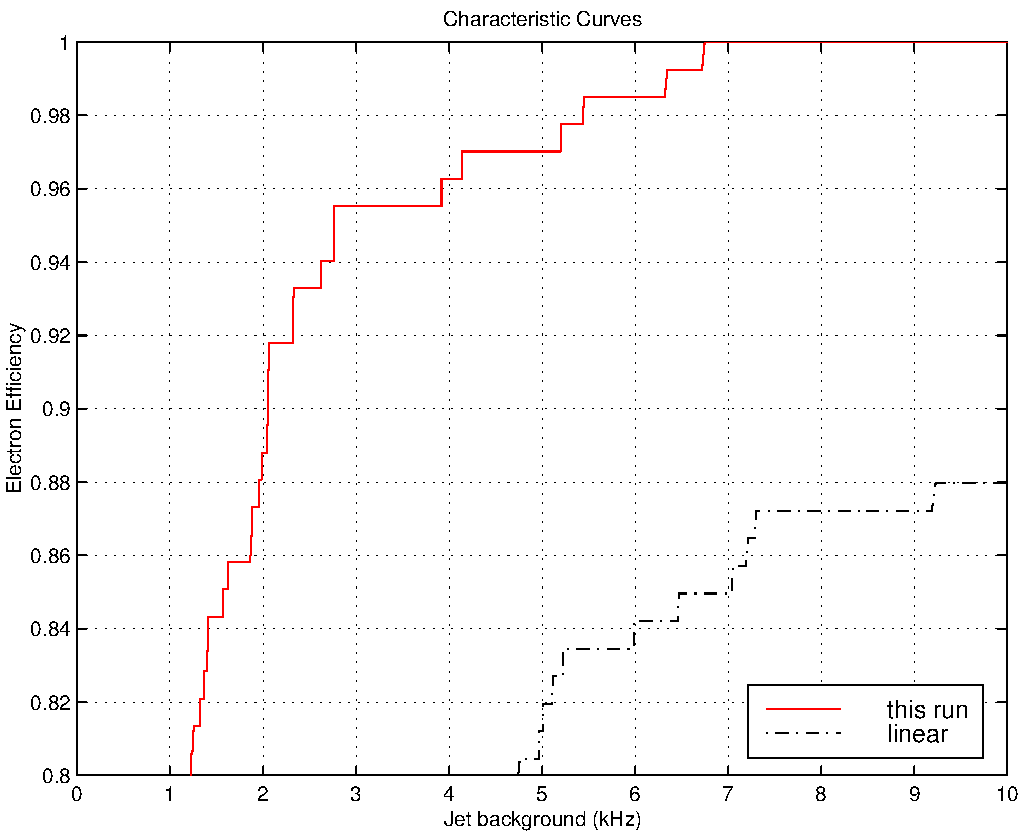
\includegraphics[scale=0.65]{msc/efficiency-3}
\end{center}
\caption{Comparação entre o discriminador linear e o neural (Teste~3).}
\label{fig:comp-linear}
\end{figure}

\begin{figure}
\begin{center}
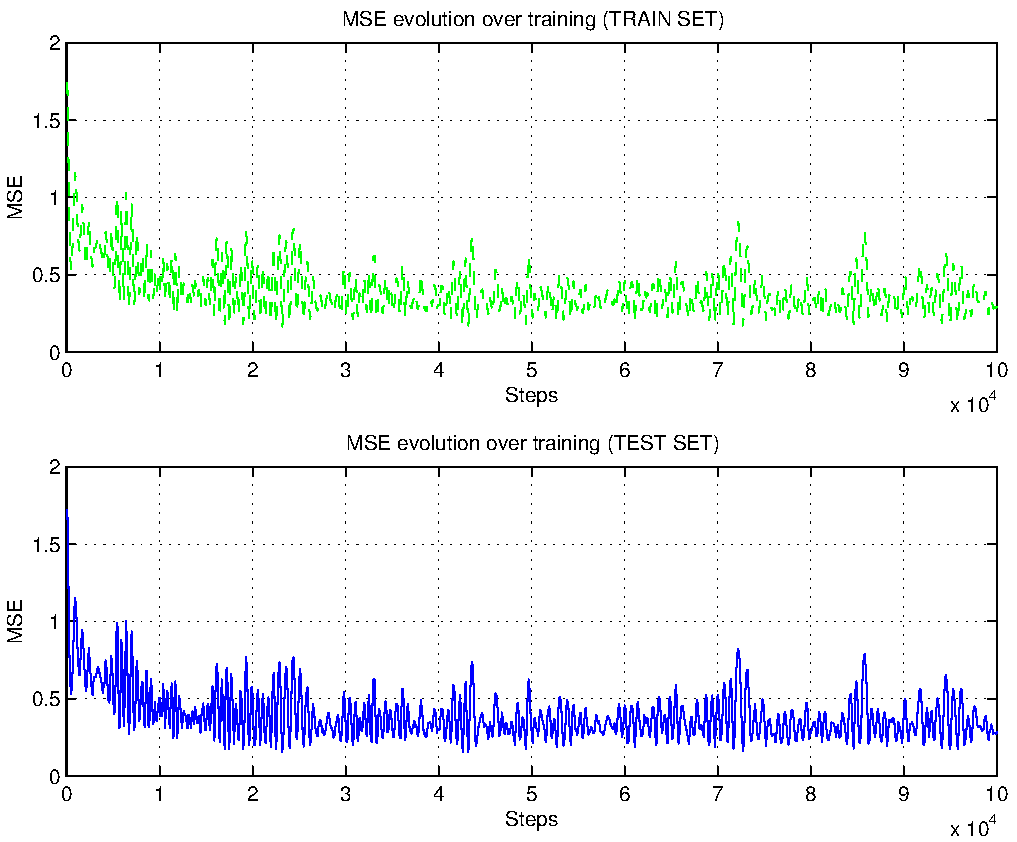
\includegraphics[scale=0.65]{msc/mse-evolution2-3}
\end{center}
\caption{Evolução do Erro Médio Quadrático durante o treinamento da rede 3.}
\label{fig:emq}
\end{figure}

\section{Compactação dos dados de entrada usando a\-néis}
\label{sec:aneis}

No processamento clássico, as cerca de 1.000 células da RoI na entrada do
discriminador são reduzidas a quatro quantidades, facilmente processáveis por
métodos clássicos ou neurais como foi visto. No entanto, desejando-se
processar em tempo real estas células, utilizando toda a granularidade
disponível, há um problema: a dimensionalidade do espaço de entrada torna
proibitivo qualquer método de discriminação direto, devido ao tempo necessário
de processamento para a operação \eng{on-line}. Por outro lado, a utilização
de toda a granularidade disponível, poder levar a maiores eficiências de
discriminação \cite{seixas:fe, andre-enfpc2000, andre-enfpc98}.

A solução para esta dificuldade pode estar numa compactação eficiente dos
dados de entrada. Neste trabalho, propõe-se uma versão modificada de
compactação em anéis descrita em \cite{seixas:sp}, que será adaptada às
condições de granularidade variante da configuração atual de calorímetros do
ATLAS \cite{aa:nima-2003}.

A compactação em anéis \cite{seixas:perf-loss, seixas:sp} aproveita-se do
isotropismo na deposição de energia por parte dos objetos que interagem com o
calorímetro. A tendência é que as partículas desenvolvam suas cascatas rumando
para o exterior dos calorímetros, com raio crescente, de forma semelhante a um
cone. A Figura~\ref{fig:cone} exemplifica o que idealmente ocorreria. As setas
ilustram o decaimento do objeto em objetos menos energéticos, enquanto este
interage com o detetor. Num detetor segmentado, é possível pressupor que este
fenômeno será observável a cada camada, representado no cone da figura por uma
de suas seções transversais.

\begin{figure}
\begin{center}
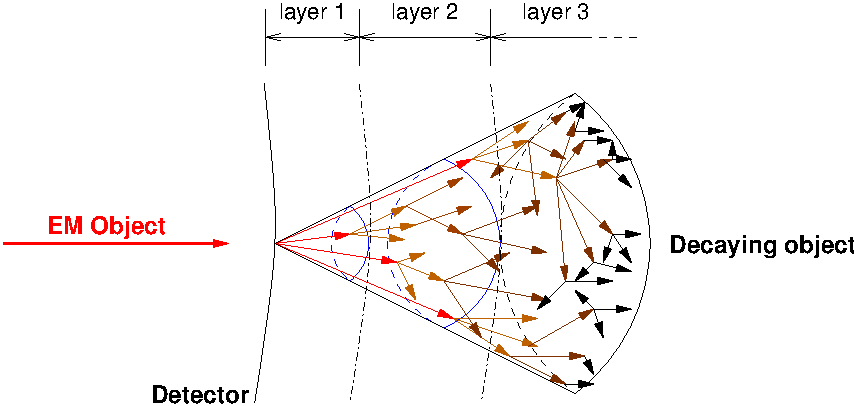
\includegraphics[scale=0.7]{msc/cone}
\end{center}
\caption{Idealização da deposição de energia.}
\label{fig:cone}
\end{figure}

Já que os calorímetros são divididos em camadas com granularidade variante, é
natural propor que cada camada tenha seu conjunto de anéis. Assim, pode-se
explorar eficientemente a informação detalhada oferecida pelos calorímetros do
ATLAS.

Os anéis de cada camada são extraídos localizando-se a célula que registrou a
maior deposição de energia na camada e somando-se o valor das células
concêntricas a este ponto. Cada conjunto de células vizinhas\footnote{Chama-se
vizinha, a célula que se encontra adjacente à parte externa de um anel.} é um
anel. A Figura~\ref{fig:ring} ilustra como extrair os anéis de algumas camadas
dos calorímetros do ATLAS. Após identificar a célula com maior deposição de
energia, procuram-se as células vizinhas que a circundam, formando um anel
\emph{quadrado}. Prossegue-se com este algoritmo, buscando o anel seguinte, até
que se esgotem todas as células na camada. Durante este processo, é possível
definirem-se anéis incompletos. Em casos extremos, como no \eng{Presampler} e
na terceira camada do calorímetro e.m., os anéis nem mesmo são
conectados. Ainda assim, os valores destes anéis incompletos são somados para
dar lugar a uma única quantidade. Por exemplo, na terceira camada do
calorímetro e.m. (na parte esquerda inferior da Figura~\ref{fig:ring}),
marcaram-se as células que somadas produzirão as quantidades de
interesse. Cada quantidade representará um anel para o discriminador. A
extração de anéis é uma atividade que deverá ser adicionada ao sistema de
pré-processamento.

\begin{figure}
\begin{center}
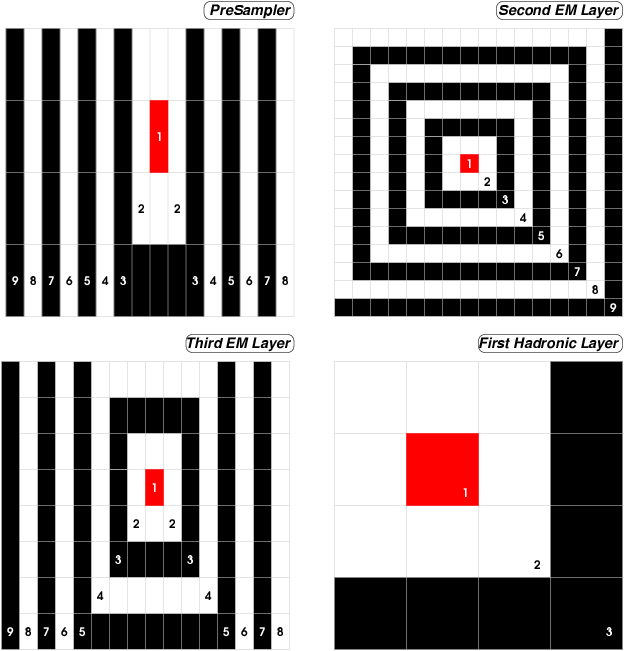
\includegraphics[scale=0.5]{msc/rings}
\end{center}
\caption{A extração de anéis em uma RoI nos calorímetros do ATLAS.}
\label{fig:ring}
\end{figure}

Construiu-se o pré-processador para os dados de simulação descritos
anteriormente. Após processadas, as cerca de 1.000 células iniciais são
reduzidas a 58 somas em anel, como organizadas na Tabela~\ref{tab:ring-org}.

\begin{table}
\caption{O número de anéis por camada do calorímetro.}
\label{tab:ring-org}
\begin{center}
\begin{tabular}{>{\bfseries}l r}
Camada & Número de Anéis \\ \hline
Pré-irradiador & 6 \\
1\eira\ camada e.m. & 33 \\
2\eira\ camada e.m. & 10 \\
1\eira\ camada Hadrônica & 3 \\
2\eira\ camada Hadrônica & 3 \\
3\eira\ camada Hadrônica & 3 \\ \hline
\end{tabular}
\end{center}
\end{table}

É perceptível que o número de anéis em algumas camadas, por exemplo no
Pré-irradiador, é menor que o necessário para extrair todas as quantidades, ou
anéis, possíveis daquela camada. No entanto, a quantidade de ruído na borda é
tipicamente grande, como é possível ver na Figura~\ref{fig:lastring}. Essa
figura mostra o histograma (normalizado para ter área unitária) dos últimos
anéis de cada camada. No eixo das abcissas é possível ver o valor energético
normalizado usando toda a energia da RoI, enquanto que no eixo das coordenadas
é possível ver a probabilidade de se ter aquele valor energético no último
anel da camada.

Desta forma, para se aproveitar a possível informação existente nestes anéis,
somam-se os valores dos últimos anéis formando uma quantidade única,
aumentando, possivelmente, a relação sinal/ruído nesta região.

\begin{figure}
\begin{center}
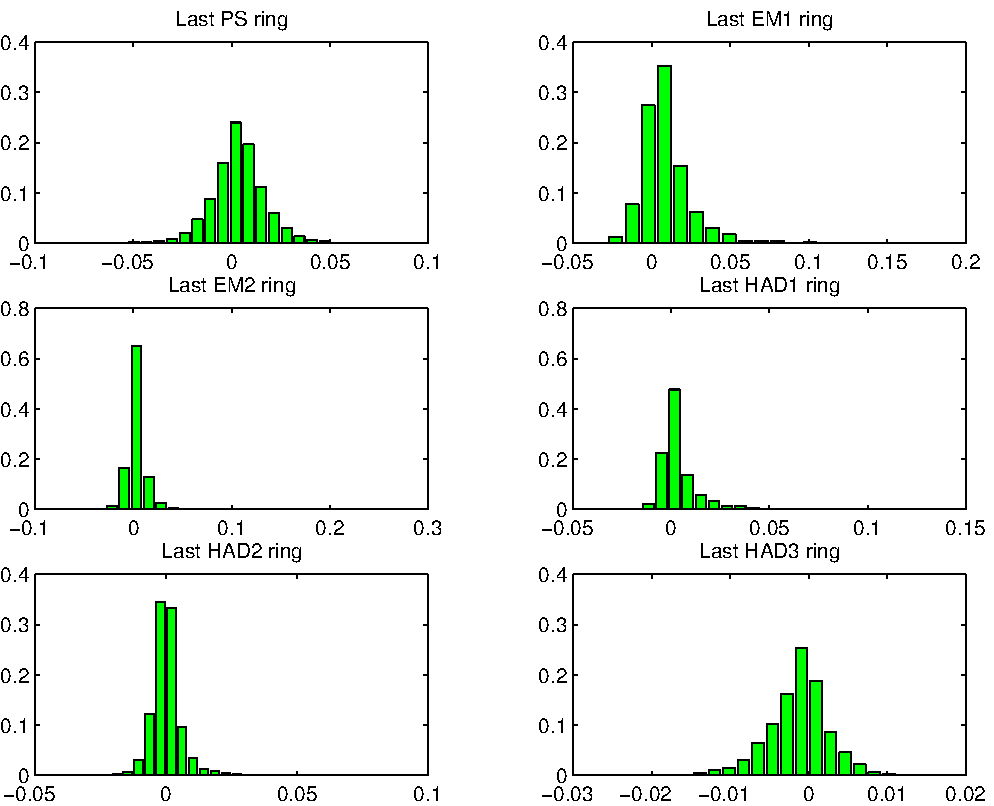
\includegraphics[scale=0.6]{msc/lastring}
\end{center}
\caption[A distribuição da energia contida nos últimos anéis de cada camada do
calorímetro (normalizada para área unitária).]{A distribuição da energia
contida nos últimos anéis de cada camada do calorímetro (normalizada para área
unitária). No eixo horizontal observa-se a energia no último anel, enquanto que
no vertical, a probabilidade de ocorrência daqueles valores energéticos.}
\label{fig:lastring}
\end{figure}

\subsection{Normalização}
\label{sec:normal}

A energia dos objetos que devem ser discriminados pode variar bastante
\cite{hlt-tdr}. As células do calorímetro respondem a esta variação influenciando
no valor de cada uma das somas (dos anéis) extraídas. Por outro lado,
classificadores neuronais são muito sensíveis a variações bruscas da amplitude
de suas entradas, podendo eventualmente vir a saturar, perdendo desempenho.

Para evitar este efeito, é possível normalizar os dados de cada RoI, tendo por
base a energia (transversa) do objeto sendo discriminado. Realizando-a, se
está, artificialmente, eliminando as diferenças energéticas entre os diversos
objetos e.m. que serão processados, permitindo que o discriminador
conecentre-se nas diferenças nos padrões de deposição energética. Esta forma
de normalização permite se obter um discriminador único para objetos com
diferentes níveis energéticos uma vez que a resolução em energia no
calorímetro melhora com o aumento da energia do objeto, espera-se que a
qualidade de discriminação melhore com a energia. Neste trabalho, a análise
está limitada à faixa de menor energia (pior caso), nas condições do ATLAS:
objetos e.m. com 20 GeV.

A normalização em energia pode ser feita de várias formas de acordo com a
segmentação do sistema de calorimetria:

\begin{description}
\item[Energia do Evento] Nesta modalidade soma-se a energia de todas as células
da RoI. Divide-se o valor de energia em cada célula da RoI pelo valor total
encontrado;

\item[Energia da Seção] Aqui divide-se o calorímetro do ATLAS em duas seções,
e.m.  e hadrônico, calculando a energia depositada em cada uma delas. Cada
célula é dividida pela energia total de sua respectiva seção;

\item[Energia da Camada] O mesmo dos dois outros tipos de normalização, mas
leva-se em consideração a energia em cada camada do calorímetro;

\item[Sequencial] Este tipo de normalização propõe um esquema de amplificação
da energia dos anéis periféricos ao 1\eiro\ anel da camada, de forma que a
informação contida nestes anéis seja realçada, possivelmente melhorando o
desempenho do discriminador.

Nesta modalidade, para cada camada, calcula-se a soma das energias de cada
célula e divide-se o valor da energia do primeiro anel por esta soma. A energia
do segundo anel é dividida pelo valor da soma menos a energia do primeiro
anel. A energia do terceiro anel, pela soma da energia total menos a energia do
primeiro e segundo anéis, e assim sucessivamente até que o número de anéis se
esgote.

Um problema ocorrerá: os valores energéticos nos últimos anéis de cada camada,
aqueles nos quais a razão sinal-ruído é a menor, terão o menor fator
normalização e, portanto, a maior amplificação. Isto é prejudicial ao
desempenho de qualquer discriminador, pois beneficiar-se-íam canais ruidosos
àqueles que realmente contêm informação relevante à discriminação. A solução é
limitar a variação do fator de normalização por camada. Assim, por exemplo, na
segunda camada e.m. somente os primeiros 7 anéis serão normalizados utilizando
este esquema variável. Os demais anéis serão normalizados por um fator
constante geralmente igual ao fator de normalização do 7\eiro\ anel. A
Tabela~\ref{tab:seq} exemplifica a execução do algoritmo. Na primeira coluna é
possível ver a posição do anel que será normalizado, na segunda o fator de
normalização e na terceira a soma em anel correspondente. Nessa situação
hipotética, há N anéis na camada e somente o os ($N-3$) primeiros serão
normalizados com o esquema variante. Os demais (a partir de $N-2$) serão
normalizados por um valor constante, igual ao fator de normalização do anel
($N-3$).

Como variantes deste processo, ao invés de se usar a energia total do objeto,
pode-se utilizar a energia da seção ou da camada, relativas ao segmento para o
qual se está aplicando a normalização, ou ainda esquemas híbridos. Ademais, a
identificação em cada camada do ponto crítico (a partir do qual a normalização
será feita de acordo a um fator constante) não é trivial
\cite{seixas:sp}. Desta forma, optou-se por não realizar o estudo com
normalização seqüencial neste trabalho, reservando-o para futuras atualizações
do mesmo.

\begin{table}
\renewcommand{\baselinestretch}{1}
\caption{Normalização sequencial.}
\label{tab:seq}
\begin{center}
\begin{tabular}{>{\bfseries}l r r}
Anel & Normalização & Soma em anel \\ \hline
1 & $E$ (total da camada) & $E_1$\\
2 & $E - E_1$ & $E_2$ \\
3 & $E - E_1 - E_2$ & $E_3$\\
4 & $E - E_1 - E_2 - E_3$ & $E_4$\\
\dots  & \dots \\
N-4 & $E - E_1 - E_2 - ... - E_{N-5}$ & $E_{N-4}$ \\
N-3 & $E - E_1 - E_2 - ... - E_{N-5} - E_{N-4}$ & $E_{N-3}$ \\
N-2 & $E - E_1 - E_2 - ... - E_{N-5} - E_{N-4}$ & $E_{N-2}$ \\
N-1 & $E - E_1 - E_2 - ... - E_{N-5} - E_{N-4}$ & $E_{N-1}$ \\
N & $E - E_1 - E_2 - ... - E_{N-5} - E_{N-4}$ & $E_N$ \\
\end{tabular}
\end{center}
\renewcommand{\baselinestretch}{1.5}
\end{table}

\end{description}

\section{Treinamento Neural}

Após compactar os dados usando a técnica de anéis, adaptada aqui para a
granularidade variada camada a camada, é possível começar a projetar nosso
discriminador neuronal. Lembrando, têm-se um conjunto de 58 somas em anel, que
estão normalizadas de acordo com cada uma das técnicas
descritas\footnote{Exceto normalização seqüencial.} na
Seção~\ref{sec:normal}. Este fato estabelece imediatamente um dos parâmetros
da rede neuronal: o número de nós de entrada. Como identificar-se-ão apenas
duas classes de objetos, apenas um nó na saída será suficiente. A função de
ativação escolhida é a tangente hiperbólica. Durante o treinamento
supervisionado por retro-propagação de erros, o alvo para elétrons será
mantido em $+1$, enquanto que para jatos, $-1$.

Um dos primeiros parâmetros a ser escolhido é, sem dúvida, o número de
neurônios na camada intermediária. Estudos com componentes principais
\cite{seixas:pca} indicam que cerca de 10 neurônios são suficientes para
realizar discriminação similar. Isto motiva testes de redes tendo entre 5 e 15
neurônios na camada intermediária (escondida).

\subsection{Critério de Parada: o produto SP}
\label{sec:sp}

O critério de parada deve estar intimamente relacionado com a finalidade do
projeto. Embora se estabeleça um conjunto de alvos, desejando que a rede
convirja para $+1$ (quando elétrons aparecerem) ou $-1$, se existirem jatos em
sua entrada, se está fundalmentalmente interessado no poder de discriminação
desta rede. Sendo assim, o erro médio quadrático pode não traduzir facilmente
tal objetivo, pois mede a distância euclidiana entre a saída do classificador
e os valores-alvo, e não diretamente o poder de discriminação da rede
neuronal. Para mediar esta dificuldade, é possível utilizar uma medida de
eficiência do classificador como critério de parada do treinamento da rede
neuronal
\cite{haykin}. 

O poder de discriminação está relacionado à eficiência com que separam-se as
duas classes de eventos. Desta forma, é necessário levar em conta os valores de
eficiência para ambas as classes, pois deseja-se que ambos atinjam o
máximo. Seria possível, por exemplo, considerar a soma de ambas as eficiências
(S). Neste caso, valores próximos de 2 representariam uma excelente separação.

Considerando a soma das eficiências como critério de parada, entretanto, seria
possível deparar com situações nas quais a eficiência de discriminação de uma
das classes é alta, mas a da outra classe é baixa. Se, por exemplo,
encontra-se o valor da soma das eficiências igual a 1,3. Isto quer dizer que a
primeira classe foi discriminada com 80\% de acerto e a segunda com 50\%?
Talvez. Isto quer dizer que as eficiências juntas somam 1,3 e nada mais. A
soma das eficiências, portanto, pode produzir eficiências de classificação não
uniforme para as duas classes de interesse, o que não é interessante nesta
aplicação, pois deseja-se atingir uma elevada eficiência de discriminação (em
elétrons) com o mais baixo nível de falso alarme (deteção errônea de jatos).

O produto das eficiências, no entanto, restringe a existência de tal
desequilíbrio, uma vez que valores baixos para a eficiência numa dada classe
implicarão em valores baixos para tal produto. Neste trabalho, conjugam-se as
duas medidas de desempenho do classificador, adotando o produto SP, i.e., a
soma vezes o produto das eficiências (equação~\ref{eq:sp}), como critério de
parada no treinamento do discriminador neuronal.

\begin{equation}
\text{SP} = (\text{efic}_{classe_1} + \text{efic}_{classe_2}) \times
(\text{efic}_{classe_1} \times \text{efic}_{classe_2})
\label{eq:sp}
\end{equation}

No método de treinamento que foi utilizado, guarda-se sempre a rede que,
durante o treinamento, apresenta o melhor produto SP, levando-se em
consideração, para um mesmo classificador, o melhor produto SP obtido
observando-se a sua curva característica ponto-a-ponto. É claro que se espera
que esta rede também apresente um baixo erro médio quadrático, embora esta
variável não seja utilizada como critério de parada no processo de treinamento
da rede. O erro médio quadrático, não obstante, é usado como função objetivo a
ser minimizada pelo processo de treinamento da rede. A título de exemplo, a
Figura~\ref{fig:emq-sp} mostra a evolução do EMQ (parte superior) e do produto
SP (parte inferior) para o conjunto de teste de uma das redes apresentadas na
Seção~\ref{sec:eff-classical}. Nessa figura, nota-se que o valor de SP de fato
aumenta com a diminuição do EMQ, ainda que não se observe uma correlação plena
entre as duas quantidades.

\begin{figure}
\begin{center}
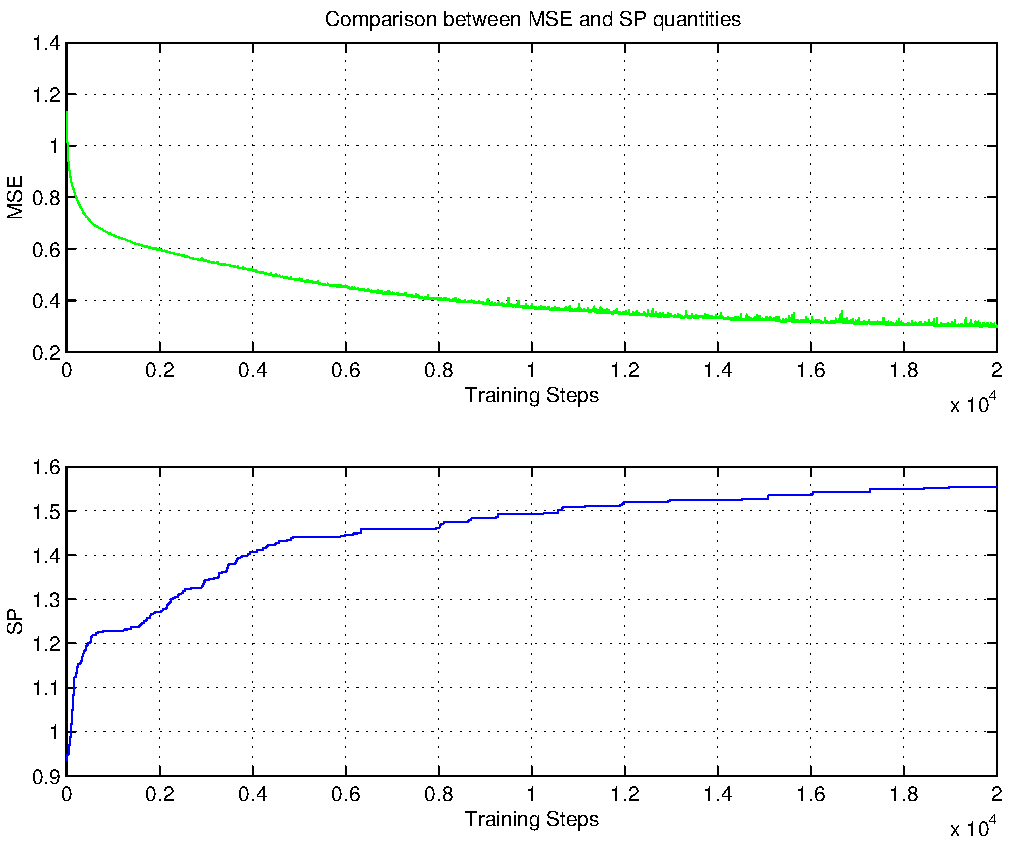
\includegraphics[scale=0.65]{msc/evolution-eg}
\end{center}
\caption{Evolução comparativa entre o EMQ e o produto SP em um treinamento
neural.}
\label{fig:emq-sp}
\end{figure}

\subsection{Treinamento}

O método de treinamento a ser adotado é a retro-propagração de erros com
momento e decaimento da taxa de treinamento, como na
Seção~\ref{sec:eff-classical}. Também serão adotados \emph{épocas de
treinamento}. O uso de \emph{épocas} atenua a oscilação durante a convergência
da rede neuronal \cite{haykin, jetnet}. O tamanho da época terá que ser
escolhido, assim como a taxa de aprendizado, seu decaimento e o momento. O
número de passos de treinamento deverá ser grande o suficiente para a
estabilização do produto SP e do erro médio quadrático.

O treinamento das redes neuronais que executarão a separação elétron/jato foi
feito dividindo-se o conjunto de dados em 2 sub-conjuntos, cada um contendo a
metade do número de eventos total. Isto se traduz em cerca de 300 elétrons e
1800 jatos para cada conjunto.

As figuras de mérito que serão utilizadas para julgar o comportamento da rede
são o EMQ para os conjuntos de treino e teste, a evolução do produto SP para os
conjuntos de treino e teste e a comparação da curva característica obtida no
classificador encontrado com a obtida pelo melhor discriminador neuronal usando
as quantidades clássicas.

\section{Resultados}

A Tabela~\ref{tab:ring-neural} resume os resultados encontrados, depois do
treinamento de cerca de 20 redes neuronais com parâmetros diferentes, para o
vetor de entrada normalizado, usando-se o enfoque de normalização pela soma
das energias de todas as células da RoI (energia total). A organização desta
tabela é semelhante a da Tabela~\ref{tab:class-neural}, com exceção da última
coluna, que define o número de neurônios escondidos usados durante o
treinamento.

\renewcommand{\baselinestretch}{1}
\begin{table}
\caption[Os resultados do treinamento de 20 redes neurais para separação
elétron/jato utilizando anéis.]{Os resultados do treinamento de 20 redes
neurais para separação elétron/jato utilizando anéis. A normalização do vetor
de entrada se utiliza da soma das energias de todas as células da RoI.}
\label{tab:ring-neural}
\renewcommand{\baselinestretch}{1.4}
\small
\begin{center}
\begin{sideways}
\begin{tabular}{|c|c|c|c|c|c|c|c|c|c|c|c|c|c|} \hline
Teste & $\mu$ & $\alpha$ & $\gamma$ & SP & \# Passos & Bat. & Itera��o & EMQ
& Patamar & \% e$^-$ & \% jatos & Tx.(kHz) & \# esc.\\
\hline\hline

1 & 0,1 & 0 & 1 & 1,72 & 2500 & 400 & 2341 & 0,206 & 0,170 & 95,38 & 94,76
& 1,31 & 15 \\ \hline

2 & 0,15 & 0 & 1 & 1,72 & 2500 & 400 & 2047 & 0,182 & 0,070 & 96,04 &
94,26 & 1,43 & 15 \\ \hline

3 & 0,15 & 0 & 0,9 & 1,72 & 2500 & 400 & 2405 & 0,154 & -0,050 & 95,71 &
94,59 & 1,35 & 15 \\ \hline

4 & 0,15 & 0 & 0,9 & 1,73 & 2500 & 200 & 1129 & 0,262 & 0,410 & 95,38 &
95,03 & 1,24 & 15 \\ \hline

5 & 0,02 & 0 & 0,95 & 1,70 & 20000 & 25 & 14365 & 0,245 & 0,180 & 95,05 &
94,43 & 1,39 & 15 \\ \hline

6 & 0,05 & 0,9 & 0,95 & 1,74 & 2000 & 100 & 1996 & 0,159 & 0,060 & 96,04 &
94,92 & 1,27 & 12 \\ \hline

7 & 0,05 & 0,9 & 0,95 & 1,75 & 3000 & 100 & 2944 & 0,213 & 0,550 & 95,05 &
96,14 & 0,97 & 12 \\ \hline

8 & 0,05 & 0,9 & 0,95 & 1,75 & 5000 & 100 & 4776 & 0,148 & -0,030 & 96,70 &
94,70 & 1,32 & 12 \\ \hline

9 & 0,05 & 0,9 & 0,95 & 1,76 & 5000 & 100 & 5000 & 0,150 & -0,230 & 98,35 &
93,38 & 1,66 & 14 \\ \hline

10 & 0,1 & 0,9 & 0,95 & 1,75 & 1000 & 100 & 741 & 0,145 & -0,010 & 96,04 &
95,14 & 1,21 & 7 \\ \hline

11 & 0,08 & 0,95 & 0,95 & 1,77 & 5000 & 100 & 3949 & 0,156 & -0,130 & 97,69
& 94,26 & 1,43 & 7 \\ \hline

12 & 0,08 & 0,95 & 0,95 & 1,77 & 5000 & 100 & 4736 & 0,129 & -0,360 & 97,36
& 94,54 & 1,37 & 8 \\ \hline

13 & 0,08 & 0,95 & 0,95 & 1,77 & 5000 & 100 & 4158 & 0,130 & -0,290 & 97,03
& 94,87 & 1,28 & 6 \\ \hline

14 & 0,12 & 0,95 & 0,95 & 1,76 & 4000 & 150 & 2633 & 0,285 & 0,690 & 97,03
& 94,70 & 1,32 & 5 \\ \hline

15 & 0,09 & 0,99 & 0,95 & 1,77 & 3000 & 200 & 2761 & 0,160 & -0,220 & 98,02
& 93,87 & 1,53 & 5 \\ \hline

16 & 0,05 & 0,99 & 0,95 & 1,76 & 5000 & 200 & 2562 & 0,109 & -0,830 &
97,36 & 94,43 & 1,39 & 5 \\ \hline

17 & 0,01 & 0,99 & 0,95 & 1,76 & 5000 & 200 & 2882 & 0,133 & -0,110 &
96,70 & 95,09 & 1,23 & 5 \\ \hline

18 & 0,09 & 0,95 & 0,8 & 1,76 & 5000 & 100 & 1632 & 0,216 & 0,400 & 96,70
& 94,92 & 1,27 & 5 \\ \hline

19 & 0,09 & 0,99 & 0,8 & 1,75 & 5000 & 200 & 3462 & 0,168 & -0,040 & 97,03
& 94,37 & 1,41 & 5 \\ \hline

20 & 0,09 & 0,9 & 0,8 & 1,76 & 5000 & 200 & 3467 & 0,162 & 0,020 & 97,03 &
94,65 & 1,34 & 5 \\ \hline


\end{tabular}

\end{sideways}
\end{center}
\end{table}
\renewcommand{\baselinestretch}{1.5}
\normalsize

Esta tabela mostra claramente que redes com muitos neurônios na camada
intermediária são mais difíceis de serem treinadas, vindo a apresentar um EMQ
acima do valor encontrado para redes com menos neurônios. Possivelmente, a
estatística disponível não tenha permitido (ao treinamento neuronal) o ajuste
adequado de tantas sinapses, já que o número de graus de liberdade do sistema
está na ordem do número de eventos disponíveis nestes casos. Por exemplo, ao
construir uma rede neuronal com 58 entradas, 15 neurônios na camada
intermediária e 1 neurônio na saída, obriga-se o treinamento a ajustar
$(15\times58)+15$ sinapses e mais 16 polarizações, ou seja, 900 diferentes
valores. Em contrapartida, o número de eventos disponível está na ordem de 2000
(300 elétrons e 1800 jatos). Embora não caracterize uma situação clássica de
\eng{over-fitting} \cite{vantrees}, pode-se esperar que haja uma maior
dificuldade no processo de treinamento usando-se mais neurônios na camada
intermediária, resultando, como é possível ver, num pior classificador. O valor
do produto SP é mais baixo que em outros testes, confirmando a tendência
apontada pelo EMQ.

A redução do número de neurônios aumentou consideravelmente as oscilações na
convergência do processo. Para atenuar estas oscilações, inseriu-se um valor
de momento diferente de zero em testes de redes cujo número de neurônios na
camada intermediária era menor que 15. Juntamente com a redução do decaimento
da taxa de treinamento para 0,95, foi possível chegar a redes com apenas 5
neurônios na camada intermediária sem degradação do desempenho, seguindo o
critério de parada (o produto SP). A evolução do EMQ nessas redes, no entanto,
ainda se mostrou muito ruidoso.

Ao diminuir o valor do decaimento para 0,8, procura-se uma convergência suave
do nosso discriminador, em direção ao mínimo que garanta o desempenho obtido
nos testes com 5 neurônios na camada intermediária. Os últimos dois testes
confirmam os resultados obtidos nos Testes~14 a 18: baixo erro médio
quadrático e alto poder de discrimação. A evolução do EMQ nestes testes se dá
de forma suave, como é possível observar na Figura~\ref{fig:smooth-mse}. Esta
figura é referente ao Teste~20.

\begin{figure}
\begin{center}
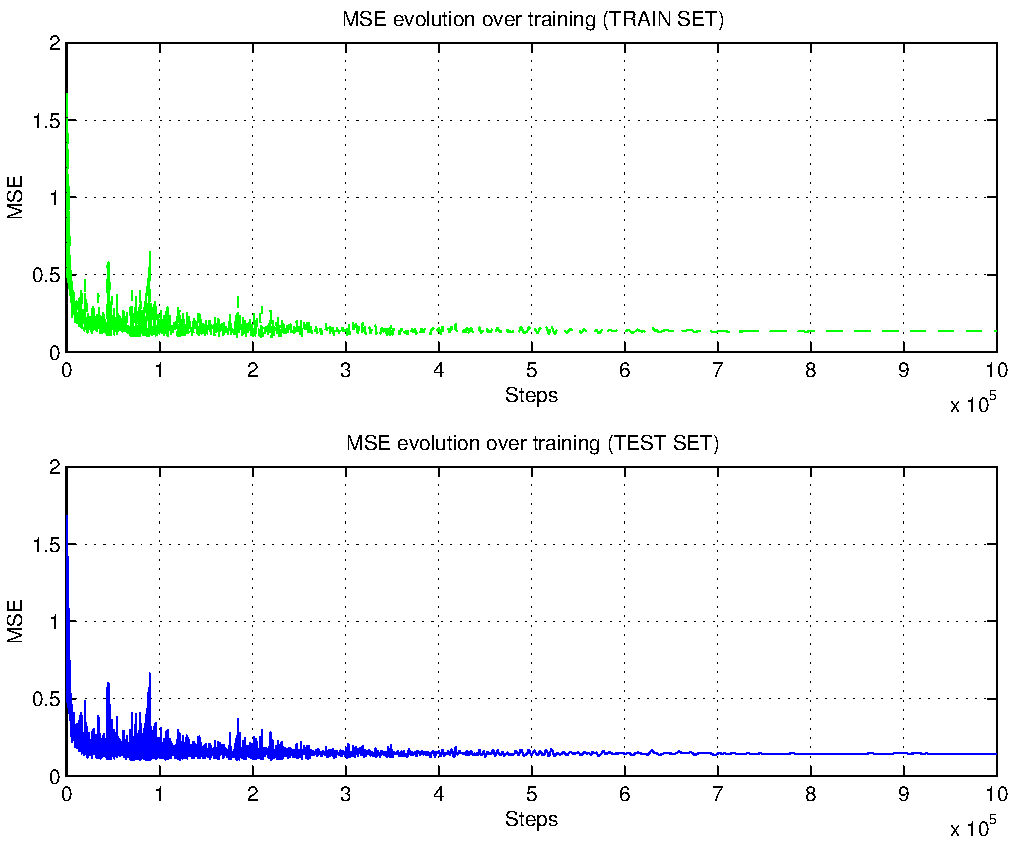
\includegraphics[scale=0.55]{msc/mse-evolution-20}
\end{center}
\caption[A evolução do EMQ para os conjuntos de treinamento (superior) e teste
(inferior) da rede neuronal cuja entrada é o vetor de anéis (Teste~20).]{A
evolução do EMQ para os conjuntos de treinamento (superior) e teste (inferior)
da rede neuronal cuja entrada é o vetor de anéis (Teste~20). A normalização do
vetor de entrada se utiliza da soma das energias de todas as células da RoI.}
\label{fig:smooth-mse}
\end{figure}

\subsection{Resultados para outras normalizações}

Testou-se também o discriminador neural se utilizando as normalizações por
camada e seção, discutidas anteriormente, sem melhoria nos resultados. De
fato, não foi possível atingir o mesmo desempenho com os dados, enquanto
normalizados a partir da energia total da RoI. A princípio, acredita-se que a
rede \emph{dê} uma importância bastante grande às diferenças energéticas entre
as duas seções dos calorímetros do ATLAS. Ao normalizar os dados de entrada
utilizando a energia da camada ou seção, se está, de fato, destruindo esta
diferença. Isso influencia no comportamento do discriminador neural, movendo-o
de seu ponto ótimo. É possível que a utilização de uma normalização híbrida
\cite{seixas:sp} nesses casos seja mais conveniente que o uso de somente um
enfoque no processo de normalização dos valores energéticos dos anéis, já que
assim beneficiam-se as diferenças de granularidade em cada camada e
respeitando suas funções no experimento. Por exemplo, o pré-irradiador é um
calorímetro muito fino e é utilizado somente para aumentar a precisão da
localização do centro da cascata do objeto. Uma normalização que utiliza toda
a energia da RoI prejudica o treinamento neuronal neste caso, à medida que
praticamente elimina a informação contida naquelas células. Este enfoque
híbrido e preocupado com as funções de cada camada do calorímetro e suas
respectivas granularidades não foi desenvolvido neste trabalho, tendo sido
reservado para investigações futuras.

A Tabela~\ref{tab:layer-section} mostra alguns resultados conseguidos
utilizando as normalizações por camadas e por seção, respectivamente. Como é
possível ver, o EMQ tende a aumentar muito quando utiliza-se esses tipos de
normalização. A utilização de mais neurônios na camada intermediária tende a
piorar o resultado. Isto confirma as tendências dos testes na
Tabela~\ref{tab:ring-neural}. Mantendo a configuração do discriminador e do
treinamento que rendeu os melhores resultados, quando utilizou-se como fator
de normalização toda a energia da RoI, os novos discriminadores gerados a
partir do treinamento com vetores normalizados pela energia da seção ou da
camada não se mostraram tão eficientes.

\renewcommand{\baselinestretch}{1}
\begin{table}
\caption[Os resultados do treinamento de algumas redes neurais usando os
58-anéis.]{Os resultados do treinamento de algumas redes neurais usando os
58-anéis. Na tabela superior mostram-se os testes utilizando a energia da
camada como fator de normalização dos dados. Na inferior, a energia da seção.}
\label{tab:layer-section}
\renewcommand{\baselinestretch}{1.5}
\small
\begin{center}
\begin{sideways}
\begin{tabular}{|c|c|c|c|c|c|c|c|c|c|c|c|c|c|} \hline
Teste & $\mu$ & $\alpha$ & $\gamma$ & SP & \# Passos & Bat. & Itera��o & EMQ
& Patamar & \% e$^-$ & \% jatos & Tx.(kHz) & \# esc. \\
\hline\hline
1 & 0.090 & 0.900 & 0.800 & 1.42 & 5000 & 200 & 4300 & 0.3880 & -0.430 & 96.37 & 82.56 & 4.36 & 5 \\ \hline

2 & 0.200 & 0.900 & 0.800 & 1.43 & 5000 & 200 & 1923 & 0.4470 & -0.170 & 97.36 & 81.90 & 4.53 & 5 \\ \hline

3 & 0.050 & 0.900 & 0.700 & 1.45 & 5000 & 200 & 4735 & 0.3820 & 0.100 & 91.09 & 88.52 & 2.87 & 5 \\ \hline

4 & 0.050 & 0.900 & 0.700 & 1.47 & 5000 & 200 & 3368 & 0.3640 & -0.080 & 94.39 & 86.31 & 3.42 & 8 \\ \hline

5 & 0.050 & 0.900 & 0.700 & 1.40 & 5000 & 200 & 3337 & 0.3710 & -0.350 & 91.42 & 86.09 & 3.48 & 12 \\ \hline

\end{tabular}

\end{sideways}
\hspace{2cm}
\begin{sideways}
\begin{tabular}{|c|c|c|c|c|c|c|c|c|c|c|c|c|c|} \hline
Teste & $\mu$ & $\alpha$ & $\gamma$ & SP & \# Passos & Bat. & Itera��o & EMQ
& Patamar & \% e$^-$ & \% jatos & Tx.(kHz) & \# esc. \\
\hline\hline
1 & 0.090 & 0.900 & 0.800 & 1.60 & 5000 & 200 & 2086 & 0.2130 & -0.070 & 93.40 & 92.44 & 1.89 & 5 \\ \hline

2 & 0.050 & 0.900 & 0.800 & 1.60 & 2500 & 200 & 1664 & 0.2880 & 0.170 & 94.06 & 91.78 & 2.06 & 5 \\ \hline

3 & 0.010 & 0.900 & 0.800 & 1.60 & 5000 & 200 & 4489 & 0.2500 & 0.130 & 92.41 & 93.10 & 1.72 & 5 \\ \hline

4 & 0.010 & 0.900 & 0.800 & 1.48 & 5000 & 200 & 4112 & 0.3140 & -0.080 & 92.08 & 88.85 & 2.79 & 10 \\ \hline

\end{tabular}

\end{sideways}
\end{center}
\end{table}
\renewcommand{\baselinestretch}{1.5}
\normalsize

\section{Informação Relevante}
\label{sec:relevance}

No ambiente de física experimental, determinar a informação relevante é de
grande importância, podendo revelar canais físicos interessantes ao
experimento. Por outro lado, conhecendo-se a informação relevante, é possível
compactar ainda mais a dimensionalidade dos sinais originais de entrada, ou
mesmo manter a informação redundante, de forma a garantir a robustez do
discriminador, em caso da ausência de alguns canais dos calorímetros.

Para identificar a informação relevante, pode se analisar a resposta do
classificador neuronal em termos da sua sensibilidade à informação contida em
cada anel. Para tal, o mapeamento de relevância \cite{relevance} mede a
variação na saída do discriminador, quando substitui-se uma componente do
vetor de entrada pelo seu valor médio. Esta operação é repetida para todos os
vetores de entrada. Tais variações são calculadas ao quadrado, somadas e
normalizadas pelo número total de padrões considerado. O valor encontrado
mede, então, a importância da variável no desempenho de saída do
classificador. A este valor dá-se o nome de \emph{relevância}. A
equação~\ref{eq:relevance} mede a relevância da i-\emph{ésima} componente de
entrada. Nessa equação, $N$ representa o número total de eventos (padrões)
disponíveis para a rede, e $x_j$ um evento particular.

\begin{equation}
R_i = \frac{1}{N} \text{ } \overset{N}{\underset{j=1}{\sum}} \text{ }
[\text{saída}(\overrightarrow{x_j}) -
\text{saída}(\overrightarrow{x_j}\mid_{x_{j,i} = \overline{x}_i})]^2 
\label{eq:relevance}
\end{equation}

\subsection{Relevância em discriminadores lineares}

A equação~\ref{eq:relevance} não leva em conta o projeto do discriminador. É
possível dessa forma aplicá-la a discriminadores lineares, ou seja, aqueles
que funcionam através da definição de patamares que melhor discriminam o
conjunto de dados de entrada, observando o espaço M-dimensional onde esses
dados se encontram.

Um discriminador linear pode ser representado por um neurônio cuja função de
ativação é a identidade. A Figura~\ref{fig:dlinear} representa os elementos que
são encontrados em um discriminador linear. A saída do discriminador é o
somatório, ponderado pelos pesos $w_i$, de todas as entradas $x_i$.

\begin{figure}
\begin{center}
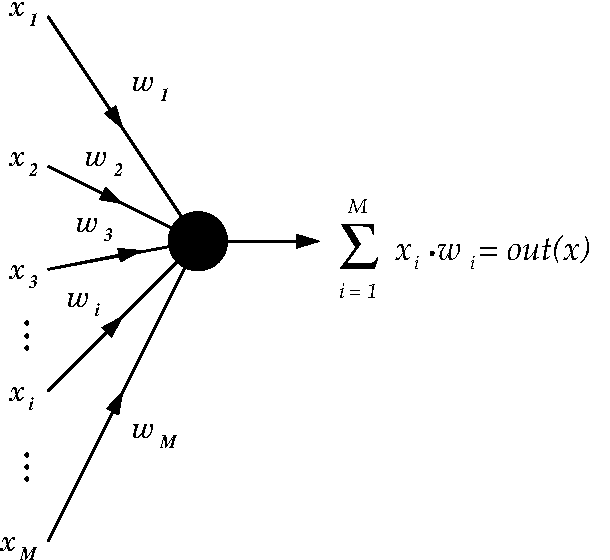
\includegraphics[scale=0.9]{msc/linear}
\end{center}
\caption{Diagrama de um discriminador linear.}
\label{fig:dlinear}
\end{figure}

Ao substituir-se uma das entradas do discriminador linear por sua média,
calcula-se a relevância desta variável. Definindo então:
\begin{align}
x_{ij} &= x_i \text{ para a j-ésima componente de entrada} \notag \\
\overline{x_i} &= E[x_i] \notag \\
y &= x^Tw \notag \\
y_i &= x\mid_{x_i=\overline{x_i}}^Tw
\end{align}

Prossegue-se com as seguintes equações:
\begin{align}
R_i &= \frac{1}{N} \text{ } \overset{N}{\underset{j=1}{\sum}} \text{ } [y_j -
y_{ji}]^2 \notag \\  
 &= \frac{1}{N} \text{ } \overset{N}{\underset{j=1}{\sum}} \text{ }
[{x_j}^Tw - {x_j}^T\mid_{x_{ij}=\overline{x_{i}}}w]^2 \notag  \\
 & = \frac{1}{N} \text{ } \overset{N}{\underset{j=1}{\sum}} \text{ }
[({x_j}^T - {x_j}^T\mid_{x_{ij}=\overline{x_i}})w]^2 \notag
\end{align}

O valor das diferenças de todos os termos de $x$, exceto o $i$-ésimo será 0,
portanto:

\begin{align}
R_i &= \frac{1}{N} \text{ } \overset{N}{\underset{j=1}{\sum}} \text{ } [(x_{ij}
- \overline{x_i})w_i]^2 \notag \\
 & = \frac{{w_i}^2}{N} \text{ } \overset{N}{\underset{j=1}{\sum}} \text{ } [x_{ij}
- \overline{x_i}]^2 \notag \\ 
 &= \frac{(N-1)\cdot{w_i}^2}{N}\cdot{\sigma_i}^2 =
{w_i}^2\cdot{\sigma_i}^2 \text{, se } N \longrightarrow \infty
\label{eq:rel-lin}
\end{align}

Ou seja, para um discriminador linear, calcular a relevância de suas entradas é
o mesmo que estimar a variância dessas entradas, quando estão ponderadas pelo
peso da sinapse que conecta cada entrada ao neurônio linear. Este resultado é
razoável, pois, para um separador linear, uma variável altamente discriminante é
aquela cuja função de densidade de probabilidade (f.d.p.) possui um domínio
bastante extenso. Uma variável que possua uma pequena variância será
inevitavelmente pouco discriminante, já que um patamar não poderá ser fixado
sem que haja uma perda muito grande em uma das classes de eventos a serem
separadas.

No caso de redes neuronais, não há como traçar um paralelo com a estatística de
forma simples, como feito com o discriminador linear, já que operações
não-lineares estão envolvidas. Não há sentido em definir a qualidade de
discriminação das classes através da variância das componentes, ainda que
cortes mais suaves possam ser esboçados em variáveis cuja variância seja
maior. Isto equivale a dizer que é mais fácil separar eventos cujas variáveis
que os representam estejam espalhadas por um grande domínio, do que separar
eventos cujas variáveis representativas possuam uma baixa variância.


\subsection{Relevância das quantidades clássicas}

A Figura~\ref{fig:class-relev} mostra o valor da relevância para cada uma das
4 quantidades clássicas, quando o mapeamento relevante é aplicado ao
discriminador do Teste~20 (Tabela~\ref{tab:class-neural}). Nessa figura,
mostra-se o valor de relevância para os conjuntos de treino e teste, de forma
que o leitor possa verificar a concordância entre os valores obtidos para os
dois agrupamentos de dados. Nesse discriminador, se obteve um alto desempenho
de discriminação associado a um baixo EMQ. De baixo para cima na figura, é
possível ver as barras de relevância para as variáveis \etem, \ethad, \rshape
e
\rstrip. É possível notar que a variável mais relevante é \ethad.

\begin{figure}
\begin{center}
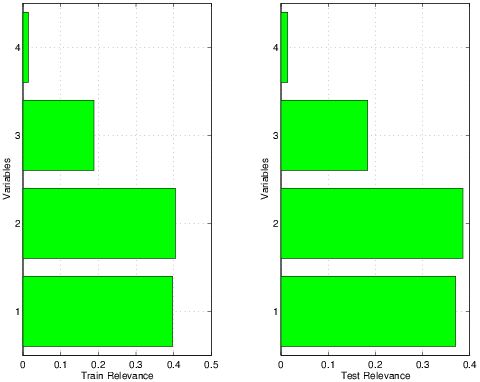
\includegraphics[scale=0.65]{msc/4neural-relevance-20}
\end{center}
\caption{Relevância as quatro quantidades clássicas no melhor discriminador
neuronal (Teste~20).}
\label{fig:class-relev}
\end{figure}

Em último lugar no quesito relevância para aquele discriminador, têm-se
\rstrip. Como foi visto nas Figuras~\ref{fig:dados-2d} e \ref{fig:dados-3d},
esta variável possui uma pequena variância, tornando-se extremamente difícil a
separação entre as duas classes de eventos. Todos os testes realizados
concordam com esta afirmação.

A Figura~\ref{fig:class-relev-worst} mostra um gráfico similar ao da
Figura~\ref{fig:class-relev}, mas tem como fonte o discriminador do Teste~18
da Tabela~\ref{tab:class-neural}. Este teste foi escolhido, uma vez que o
discriminador gerado ali apresenta baixa eficiência de discriminação e alto
EMQ, comparando-se aos dos outros testes. Como é possível ver, a relevância da
quantidade 1 (\etem) é bem menor para este discriminador que no Teste~20,
enquanto que a quantidade \ethad passa a ser muito mais relevante aqui. Este
desequilíbrio possivelmente influenciou o desempenho do discriminador, ainda
que uma análise dos eventos erroneamente classificados pelos dois
discriminadores não mostrasse qualquer tendência.

\begin{figure}
\begin{center}
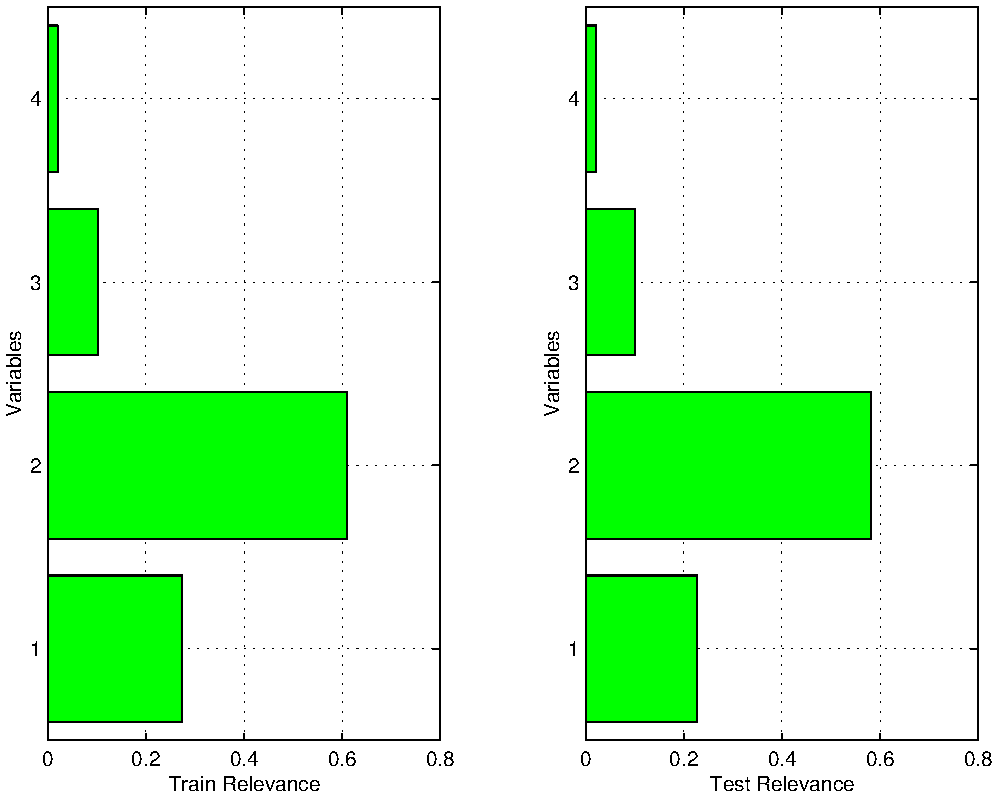
\includegraphics[scale=0.65]{msc/4neural-relevance-18}
\end{center}
\caption{Relevância das quatro quantidades clássicas no pior discriminador
neuronal (Teste~18).}
\label{fig:class-relev-worst}
\end{figure}

\subsection{Relevância dos anéis na separação neuronal}

Aplicou-se o estudo de relevância aos discriminadores baseados em anéis. A
Figura~\ref{fig:relevs} mostra, empilhadas, as relevâncias dos anéis para os
melhores discriminadores cujos fatores de normalização baseiam-se na energia
total da RoI (Teste~17), na energia da camada (Teste~4) e na energia da seção
(Teste~1), respectivamente. Os valores, de baixo para cima, representam as
relevâncias de:

\begin{center}
\begin{tabular}{>{\bfseries}l r}
Camada & Numeração \\ \hline
Pré-irradiador & de 1 a 6 \\
1\eira\ camada e.m. & de 7 a 39 \\
2\eira\ camada e.m. & de 40 a 49 \\
1\eira\ camada Hadrônica & de 50 a 52 \\
2\eira\ camada Hadrônica & de 53 a 55 \\
3\eira\ camada Hadrônica & de 56 a 58 \\ \hline
\end{tabular}
\end{center}

\begin{figure}
\begin{center}
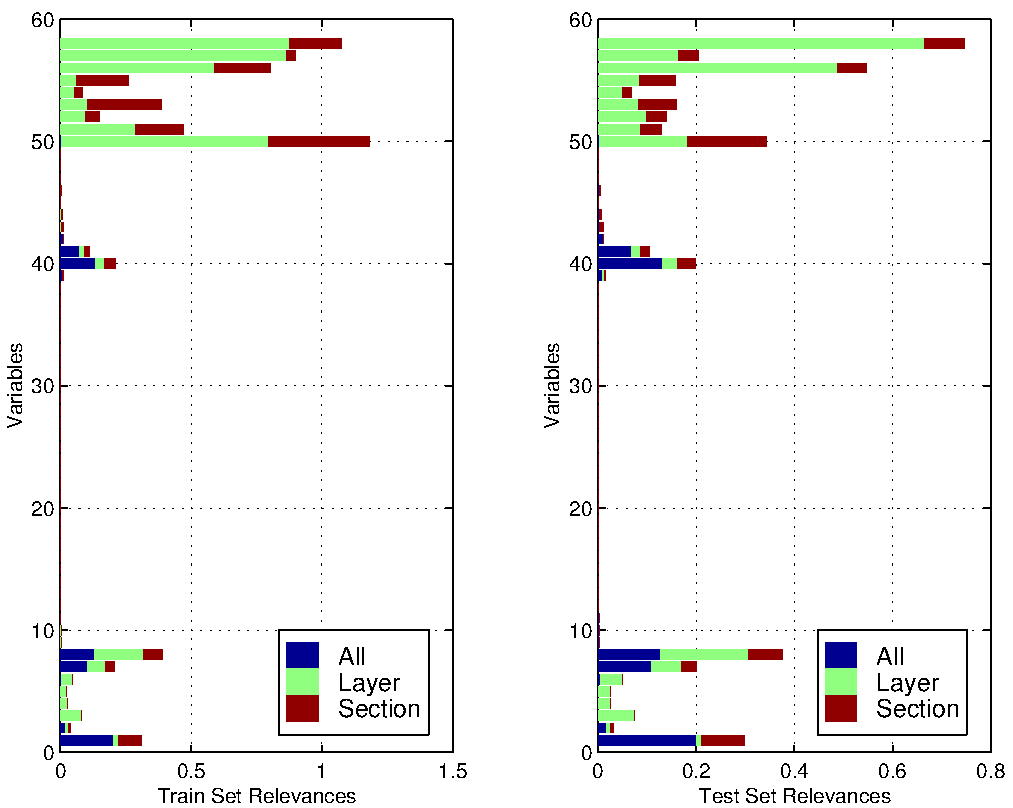
\includegraphics[scale=0.7]{msc/relevance}
\end{center}
\caption{Relevância dos 58 anéis utilizando vários tipos de normalização.}
\label{fig:relevs}
\end{figure}

Nesta figura, observa-se que o discrimador, cuja entrada é normalizada pela
energia total da RoI, dá bastante importância ao centro de energia no
Pré-irradiador, ao centro energético (1\eiro\ anel) e ao segundo anel na
primeira camada e ao primeiro e segundo anéis da segunda camada e.m.. Os
discriminadores cujas entradas são normalizadas pela energia da camada e
energia de seção valorizam notavelmente de forma mais intensa a deposição de
energia nos anéis da seção hadrônica. 

A figura~\ref{fig:haddep} mostra a deposição de energia nas camadas da seção
hadrônica para objetos e.m. (elétrons e jatos). É possível ver que, para
elétrons, a deposição de energia é praticamente nula. A flutuação que é
percebida é devida ao ruído instrumental nas camadas (subtraída de fatores de
correção). Para jatos, mostra-se o gráfico truncado, já que a cauda da
distribuição não seria observada corretamente na visão normal: há um pico cuja
altura está na casa dos milhares. Embora seja aproximadamente nula a energia
depositada na seção hadrônica para a maioria dos jatos, alguns desses podem
vir a depositar energia nestas camadas. Quando o fazem, são facilmente
discrimináveis de elétrons.

\begin{figure}
\begin{center}
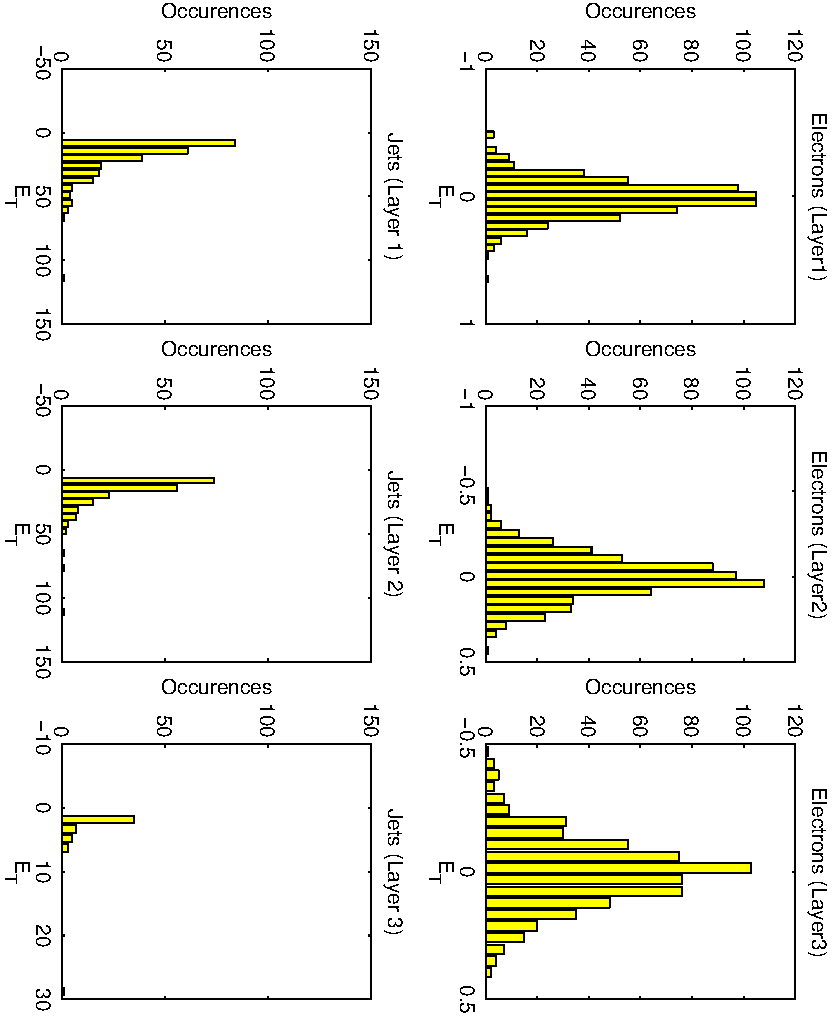
\includegraphics[scale=0.80,angle=90]{msc/hadronic-deposition}
\end{center}
\caption{A deposição de energia nas 3 camadas hadrônicas, por objetos e.m. que
representam elétrons (em cima) e jatos (embaixo).}
\label{fig:haddep}
\end{figure}

Conclui-se que a normalização baseada na energia da seção ou na energia da
camada onde se encontra a célula amplifica em demasiado o ruído contido nas
camadas da seção hadrônica. Isso piora em muito a eficiência de discriminação
entre elétrons e jatos, já que a maioria das RoI's não possui informação nestas
camadas. É importante frisar, no entanto, que a seção hadrônica contém alguma
informação de discriminação, possivelmente contida no pico de sua primeira
camada. De fato, ao se redesenhar a relevância para os dados de entrada do
discriminador que utiliza como fator de normalização a energia contida na RoI,
percebe-se que a quantidade 50 (1 anel na primeira camada hadrônica) não é
totalmente irrelevante (vide Figura~\ref{fig:relev-all}).

\begin{figure}
\begin{center}
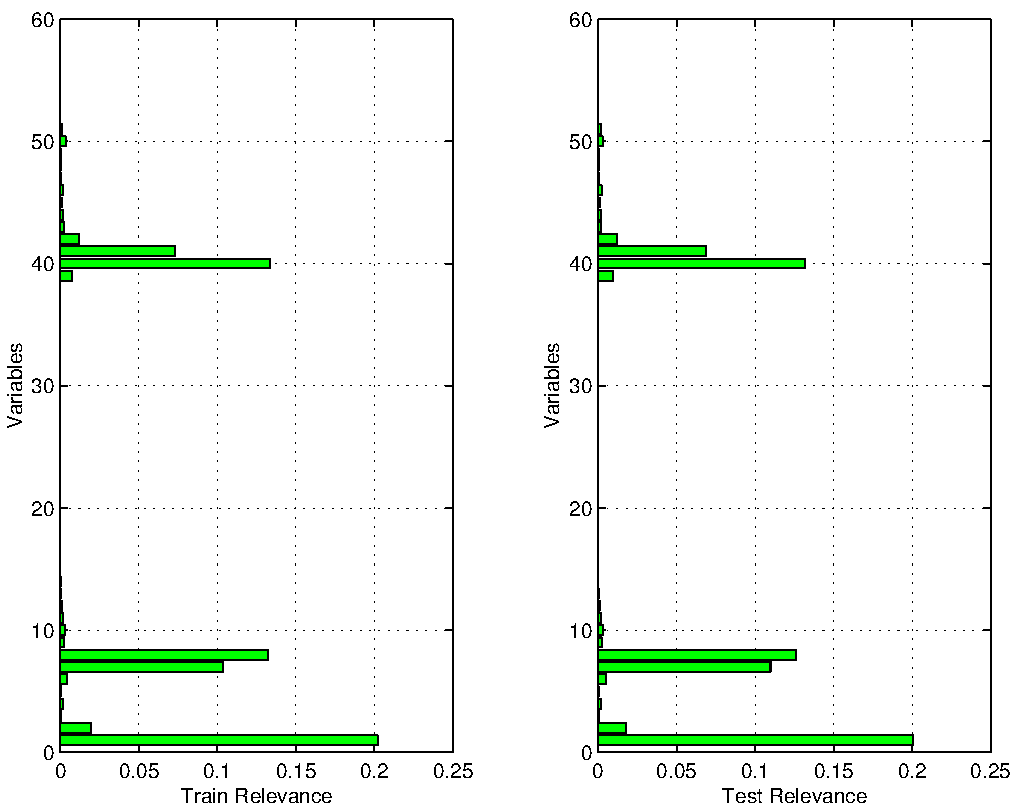
\includegraphics[scale=0.65]{msc/all-relevance-17}
\end{center}
\caption{Relevância para o Teste~17 (Tabela~\ref{tab:ring-neural}).}
\label{fig:relev-all}
\end{figure}

As diferenças nos valores de relevância entre os discriminadores baseados em
anéis e nas quatro quantidades são marcantes. No primeiro, a discriminação
baseia-se nos perfis de deposição nos centros energéticos da seção
e.m. basicamente, enquanto que no segundo há uma distribuição de
\emph{responsabilidades} entre o valor energético depositado na seção e.m. e na
seção hadrônicas. Provavelmente a construção da variável \ethad atenue os
efeitos de ruído naquela seção, tornando-a altamente discriminante. Por outro
lado, possivelmente, a deposição de tamanha responsabilidade em uma variável
extremamente ruidosa acabe por degradar, em algumas unidades percentuais, o
desempenho do discriminador usando as quatro quantidades clássicas.

\subsection{Cortes de dimensionalidade baseados na rele\-vân\-cia}

Embora apresente um melhor desempenho, o discriminador neuronal que utiliza os
anéis montados a partir da RoI, representa uma opção potencialmente lenta para
L2, já que a montagem dos anéis e o processamento neuronal são atividades mais
elaboradas que a extração das quatro quantidades clássicas e a execução de um
algoritmo de separação bi-dimensional baseado em cortes. Ainda assim, este
método apresenta uma robustez intrinsicamente maior, já que utiliza um maior
número de variáveis na discriminação, adicionando redundância ao sistema.

A partir do estudo de relevâncias, um método de \emph{poda} de rede é proposto:
dado um patamar, eliminar-se-á, da entrada, todas as variáveis cuja relevância
seja menor que o patamar. Treina-se uma nova rede neuronal mais compacta, para
que aprenda a separar elétrons e jatos utilizando somente as variáveis que
restaram.

Espera-se que a eficiência de discriminação com este processo de poda não se
deteriore de forma muito acentuada. De fato, espera-se que a robustez do
classificador seja suficientemente grande, para que se possa suprir com a
deficiência inserida no sistema. Por outro lado, espera-se estar eliminando
informação potencialmente ruidosa (das bordas do objeto predominantemente) e
não seria inesperado que a eficiência de discriminação da rede aumentasse após
o retreinamento.

\subsubsection{As variáveis clássicas}

Inicialmente, o método de redução de dimensionalidade do vetor de entrada será
aplicado ao discriminador neuronal que é alimentado pelas quatro quantidades
clássicas. A poda, neste caso, é óbvia: eliminar-se-á a variável \rstrip, que
tem a menor relevância. A dimensionalidade dos dados de entrada cairá, desta
forma, de 4 para 3.

Para se treinar a nova rede neuronal, utilizar-se-á, inicialmente, a
configuração do Teste~3 da Tabela~\ref{tab:class-neural}, variando-a até
atingir-se o desempenho equivalente a esse teste. Utilizaram-se os resultados
deste teste, pois conjuga o maior valor de produto SP na tabela, um patamar de
separação aproximadamente em zero (indicando boa separação das classes) e um
baixo erro médio quadrático, comparando-se com os outros resultados naquela
tabela.

A variação do número de neurônios na camada escondida poderá, eventualmente,
melhorar o desempenho da rede, pois garantirá um maior espaço de acomodação
para os dados, quando projetados na saída dessa camada. Lembram-se que a saída
da camada intermediária para cada padrão de entrada pode ser entendida como um
vetor que está no interior do hipercubo cuja dimensão é igual ao número de
neurônios daquela camada. Um pequeno aumento no número de neurônios na camada
intermediária, portanto, aumenta a área disponível para a acomodação dos
padrões de entrada, facilitanto o posicionamento do plano separador que será
traçado pelo neurônio na saída do classificador neuronal.

A Tabela~\ref{tab:class-relev} resume os resultados obtidos. A
Figura~\ref{fig:class-relev-best} mostra a curva de eficiência obtida no
Teste~4 (cut-34). Este corte é baseado nas relevâncias obtidas no Teste~3,
mostradas na Figura~\ref{fig:class-relev}, quando o patamar de eliminação é
0,2, i.e., eliminando a componente \rstrip.

Como é possível ver nesta figura (\ref{fig:class-relev-best}), a curva de
eficiência está, para a maior parte da abscissa, abaixo da curva anterior, mas
acima da curva gerada por um discriminador linear. Entretanto, o ponto com
maior produto SP está muito próximo da curva de eficiência obtida para o teste
utilizando as 4 componentes clássicas, indicador de que o desempenho é
compatível com os discriminadores neuronais que utilizam o espaço completo de
variáveis clássicas. O número de neurônios na camada escondida para este teste
teve que ser aumentado de 4 para 5. Isso representa um acréscimo no número de
operações para discriminação de 4 multiplicações e uma tangente hiperbólica,
mas a eliminação desta quarta variável reduz a complexidade de
pré-processamento das características do objeto e.m., tornando desnecessária a
procura de picos na primeira camada e.m. e uma divisão.

\begin{figure}
\begin{center}
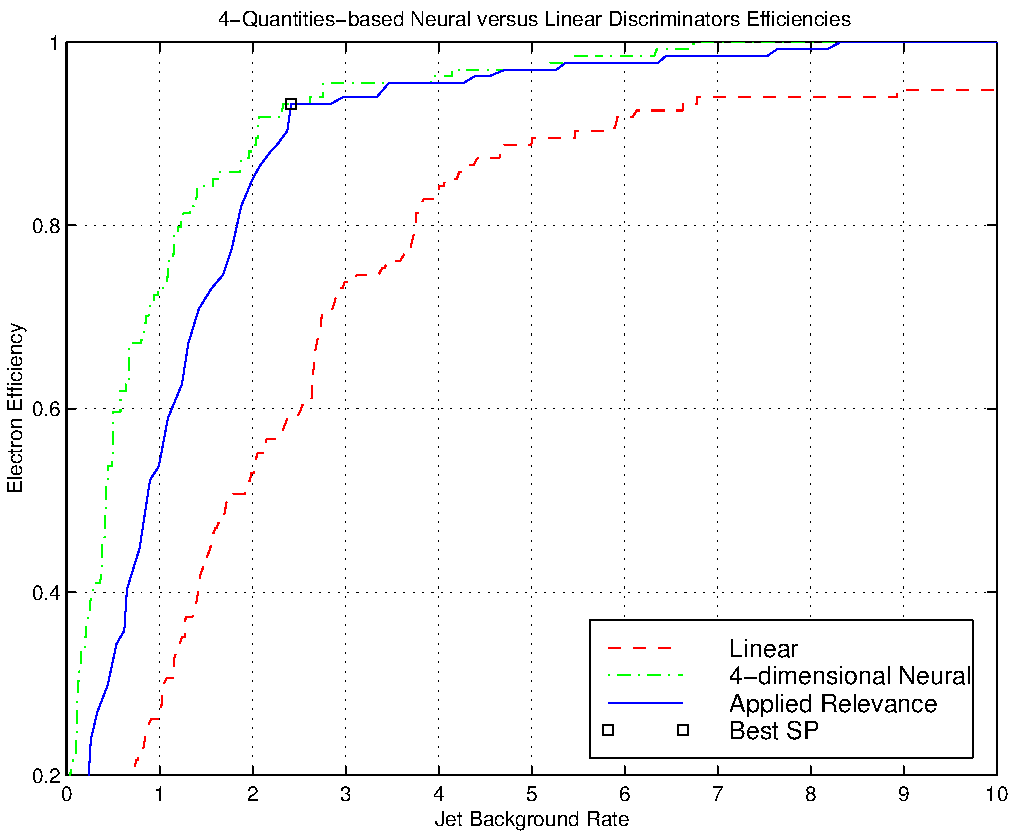
\includegraphics[scale=0.6]{msc/class-efficiency-cut-34}
\end{center}
\caption[Eficiência comparada entre o discriminador linear e os discriminadores
neuronais.]{Eficiência comparada entre o discriminador linear e os
discriminadores neuronais operando com as quatro quantidades clássicas e com o
vetor reduzido de entradas, tri-dimensional.}
\label{fig:class-relev-best}
\end{figure}

\renewcommand{\baselinestretch}{1}
\begin{table}
\caption[Resultados obtidos com algumas redes neuronais cujo vetor de entrada
são as componentes clássicas de discriminação.]{Resultados obtidos com algumas
redes neuronais cujo vetor de entrada são as componentes clássicas de
discriminação. A quarta componente (\rstrip) foi eliminada do vetor de entrada,
que agora é tri-dimensional.}
\label{tab:class-relev}
\renewcommand{\baselinestretch}{1.5}
\small
\begin{center}\begin{sideways}
\begin{tabular}{|c|c|c|c|c|c|c|c|c|c|c|c|c|c|} \hline
Teste & $\mu$ & $\alpha$ & $\gamma$ & SP & \# Passos & Bat. & Itera��o & EMQ
& Patamar & \% e$^-$ & \% jatos & Tx.(kHz) & \# esc. \\
\hline\hline
cut-31 & 0.050 & 0.900 & 0.800 & 1.54 & 1000 & 100 & 719 & 0.2510 & -0.030 & 93.28 & 90.07 & 2.48 & 4 \\ \hline

cut-32 & 0.050 & 0.700 & 0.800 & 1.55 & 1000 & 100 & 655 & 0.4870 & 0.340 & 93.28 & 90.40 & 2.40 & 5 \\ \hline

cut-33 & 0.050 & 0.500 & 0.800 & 1.55 & 1000 & 100 & 960 & 0.4920 & 0.310 & 93.28 & 90.29 & 2.43 & 5 \\ \hline

cut-34 & 0.050 & 0.500 & 0.800 & 1.55 & 1500 & 100 & 973 & 0.4630 & 0.280 & 93.28 & 90.34 & 2.41 & 5 \\ \hline

cut-35 & 0.050 & 0.500 & 0.800 & 1.51 & 1500 & 100 & 1491 & 0.4620 & 0.360 & 93.28 & 88.91 & 2.77 & 7 \\ \hline

\end{tabular}

\end{sideways}
\end{center}
\end{table}
\renewcommand{\baselinestretch}{1.5}
\normalsize

\subsubsection{Eliminando anéis}

O prosseguimento natural é aplicar os cortes de dimensionalidade baseados na
relevância em discriminadores que utilizam os anéis. Reduzindo-se o número de
anéis de entrada para o discriminador, sem perda de desempenho, se reduz a
carga computacional do pré-processamento de dados. Por outro lado, é possível
ver através da Figura~\ref{fig:relev-all} que grande parte do vetor de entrada
é pouco relevante para a rede. Neste caso, a eliminação destes anéis não
representará somente um ganho no tempo de pré-processamento dos dados, mas
também no tempo de processamento do classificador neuronal, que efetuará menos
produtos internos.

Para realizar este estudo, utilizou-se o Teste~17 da
Tabela~\ref{tab:ring-neural}, considerando-o o melhor resultado de
discriminação até aqui alcançado. A relevância de cada uma das 58 componentes
de entrada já foi discutida e pode ser vista na Figura~\ref{fig:relev-all}. É
possível selecionar vários patamares diferentes neste caso. Estes patamares nos
levarão a cortes mais severos, ou não, no número utilizado de anéis. Neste
trabalho, dois métodos para o corte de dimensionalidade dos dados de
entrada são propostos:

\begin{itemize}
\item Corte seqüencial - define-se um patamar conservador, reduz-se o conjunto
de variáveis de entrada e nova análise de relevância é feita. Um novo corte é
feito e assim é feito sucessivamente até que o desempenho do discriminador
apresente degradação acentuada. Em outras palavras, analisa-se o novo conjunto
de dados com relação à sua relevância para o melhor discriminador neuronal
encontrado. É possível aplicar um novo corte e re-análise ou parar, se houver
uma queda muito grande no desempenho. Este procedimento de re-análise permite
que a relevância das variáveis, que foram mantidas, seja reavaliada.

\item Corte direto - a partir da análise inicial de relevância, usando-se os 58
anéis, é possível estabelecer cortes mais severos, reduzindo o número de
componentes de entrada.
\end{itemize}

\paragraph{Corte seqüencial} Estabeleceu-se, inicialmente, um corte
em 0,001. Este corte poupará apenas 20 das 58 variáveis iniciais. Estas
variáveis estão listadas na Tabela~\ref{tab:left1}. Como é possível ver, a
maior parte das variáveis que restaram pertencem ao calorímetro e.m.. Este
resultado corresponde ao seguinte: na maior parte dos dados, no calorímetro
hadrônico a relação sinal/ruído é baixa, ou seja, há pouca informação
relevante à discriminação, considerando a maior parte dos dados que se
possui\footnote{De fato, este método de compactação não leva em conta que
alguns dos eventos podem ser bem discriminados usando a informação da seção
hadrônica.}.

\begin{table}
\caption{As variáveis do espaço original de anéis de dimensão 58, após o corte
baseado na relevância.}
\label{tab:left1}
\renewcommand{\baselinestretch}{1}
\begin{center}
\small
\begin{tabular}{|c|l|} \hline
Calorímetro & Anéis Restantes \\ \hline \hline
Pré-irradiador & 1, 2, 4 e 6 \\ \hline
1\eira\ camada e.m. & 7, 8, 9, 10, 11, 12 e 39 \\ \hline
2\eira\ camada e.m. & 40, 41, 42, 43, 44, 45 e 46 \\ \hline
1\eira\ camada hadrônica & 50 e 51 \\ \hline
\end{tabular}
\normalsize
\renewcommand{\baselinestretch}{1.5}
\end{center}
\end{table}

A Tabela~\ref{tab:cut-relev-ring} resume alguns resultados obtidos após o
treinamento de redes neuronais baseadas no vetor de entrada, descrito na
Tabela~\ref{tab:left1}. A Figura~\ref{fig:eff-cut1} mostra a curva de
eficiência de um dos testes desta tabela (Teste~6). O resultado é bastante
semelhante ao original (Teste~17). No entanto, utiliza-se um sub-espaço dos
dados de entrada e 1 neurônio a menos na camada intermediária, o que
representa um ganho computacional significativo. Percebe-se através desta
tabela, que o erro médio quadrático pouco se altera em relação aos testes da
Tabela~\ref{tab:ring-neural}, que utilizavam todo o espaço de entrada (os 58
anéis). Um dos discriminadores, o do Teste~8, utiliza somente 3 neurônios na
camada intermediária, sua curva de eficiência também foi bastante próxima a
curva do discriminador do Teste~17 da Tabela~\ref{tab:ring-neural}, ainda que
o EMQ atingido ao final do treinamento não tivesse sido o menor de todos na
Tabela~\ref{tab:cut-relev-ring}.

\begin{table}
\caption{Resultados de alguns discriminadores neuronais utilizando o espaço
reduzido de anéis (dimensão 20).}
\label{tab:cut-relev-ring}
\begin{center}
\small
\renewcommand{\baselinestretch}{1}
\begin{sideways}
\begin{tabular}{|c|c|c|c|c|c|c|c|c|c|c|c|c|c|} \hline
Teste & $\mu$ & $\alpha$ & $\gamma$ & SP & \# Passos & Batelada & Itera��o & EMQ
& Patamar & \% e$^-$ & \% jatos & Tx.(kHz) & \# esc. \\
\hline\hline
1 & 0.010 & 0.990 & 0.950 & 1.75 & 5000 & 200 & 4746 & 0.1720 & -0.170 & 98.02 & 93.32 & 1.67 & 5 \\ \hline

2 & 0.010 & 0.900 & 0.950 & 1.74 & 5000 & 200 & 4763 & 0.1670 & 0.030 & 96.04 & 94.92 & 1.27 & 5 \\ \hline

3 & 0.010 & 0.900 & 0.950 & 1.73 & 5000 & 200 & 4025 & 0.2030 & 0.150 & 96.37 & 94.26 & 1.43 & 6 \\ \hline

4 & 0.010 & 0.900 & 0.950 & 1.73 & 5000 & 200 & 4857 & 0.1760 & 0.150 & 95.38 & 95.09 & 1.23 & 4 \\ \hline

5 & 0.020 & 0.900 & 0.950 & 1.73 & 5000 & 200 & 3494 & 0.1630 & 0.110 & 95.38 & 95.14 & 1.21 & 4 \\ \hline

6 & 0.020 & 0.900 & 0.950 & 1.73 & 5000 & 200 & 3628 & 0.1490 & 0.030 & 95.38 & 95.25 & 1.19 & 4 \\ \hline

7 & 0.020 & 0.900 & 0.900 & 1.73 & 5000 & 200 & 4653 & 0.1840 & 0.230 & 95.38 & 95.20 & 1.20 & 4 \\ \hline

8 & 0.020 & 0.900 & 0.950 & 1.72 & 5000 & 200 & 4998 & 0.1740 & 0.070 & 95.71 & 94.43 & 1.39 & 3 \\ \hline

\end{tabular}

\end{sideways}
\normalsize
\renewcommand{\baselinestretch}{1.5}
\end{center}
\end{table}

\begin{figure}
\begin{center}
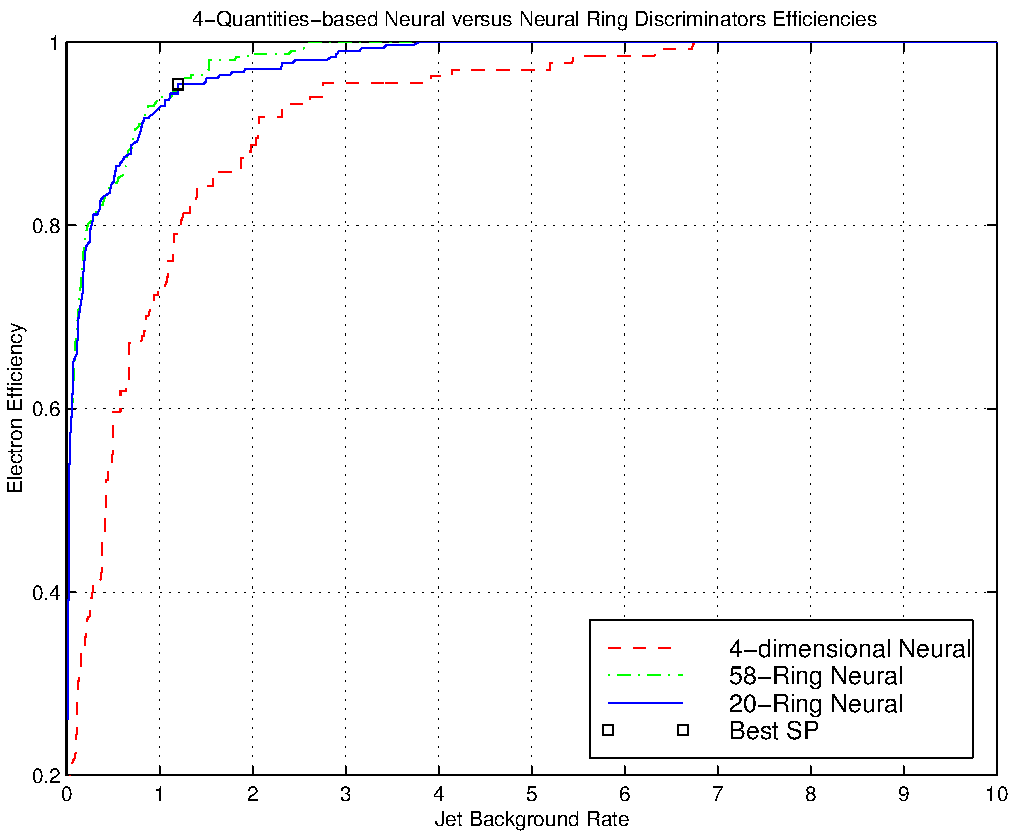
\includegraphics[scale=0.65]{msc/efficiency-cut-17-7}
\end{center}
\caption{Eficiência comparada entre os melhores discriminadores neuronais
usando os 58 anéis, 20 dos 58 anéis e as quatro quantidades clássicas.}
\label{fig:eff-cut1}
\end{figure}

Para prosseguir com os cortes na dimensionalidade do espaço de entrada,
selecionou-se o discriminador do Teste~6, pois além de apresentar o menor
valor de EMQ obtido nos testes, apresenta também alta eficiência. A partir
desse discriminador, recalcularam-se as relevâncias das entradas para o
discriminador neuronal. A Figura~\ref{fig:rel-cut1} mostra o resultado destes
cálculos. As entradas foram renumeradas neste gráfico, de forma que a primeira
quantidade apontada na Tabela~\ref{tab:left1} equivale a entrada 1, a segunda
a entrada 2 e assim sucessivamente. A última variável (o anel número 51)
equivale a 20\eira\ entrada. Este gráfico mostra que as variáveis no
calorímetro hadrônico são mais relevantes do que se pensou incialmente, quando
se estudou o primeiro gráfico de relevâncias. Isso está de acordo com a física
do experimento, já que jatos são bem discriminados quando há parte
significativa da energia do objeto na seção hadrônica.

\begin{figure}
\begin{center}
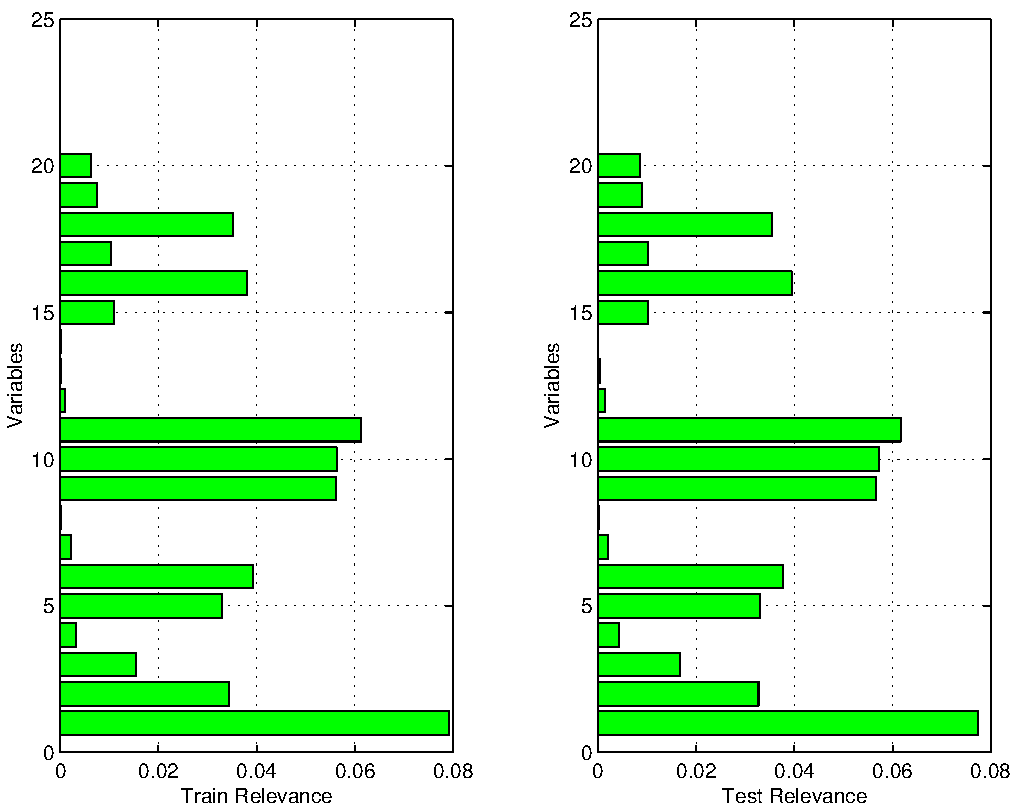
\includegraphics[scale=0.65]{msc/relevance-cut-17-7}
\end{center}
\caption{As relevâncias para os 20 anéis remanescentes do corte de
dimensionalidade do espaço de entrada original.}
\label{fig:rel-cut1}
\end{figure}

Este gráfico também mostra que algumas das variáveis que são utilizadas são,
possivelmente, supérfluas. Alguns testes eliminando diferentes quantidades de
variáveis foram realizados. A Tabela~\ref{tab:left2} resume os resultados e
configurações desses testes. Esta tabela é um pouco diferente das anteriores,
pois inclui a dimensionalidade do vetor de entrada junto com o número de
neurônios escondidos na coluna ``\emph{\# ent-esc}''. Percebe-se que o EMQ
mantém-se baixo em todos os testes, mas que a capacidade de discriminação, aqui
avaliada pelo produto SP, diminui bastante com a redução da dimensionalidade da
entrada. A Tabela~\ref{tab:config-left2} mostra os anéis que não foram podados
e portanto servem de entrada para os discriminadores da Tabela~\ref{tab:left2}.

\begin{table}
\caption{As variáveis do espaço original de anéis de dimensão 58, após o corte
baseado na relevância aplicado ao Teste~6 (Tabela~\ref{tab:cut-relev-ring}).}
\label{tab:config-left2}
\renewcommand{\baselinestretch}{1}
\begin{center}
\small
\begin{tabular}{||c||c||l||l||} \hline
\hhline{|t:=:t:=:t:=:t:=:t|}
Patamar & \# An�is & Calor�metro & An�is Restantes \\
\hhline{|:=::=::=::=:|}

\multirow{4}{35pt}{$0,0005$} & \multirow{4}{30pt}{$17$} &
\eng{Presampler} & 1, 2, 4 e 6 \\
\hhline{||~||~||-||-||}
& & 1\eira\ camada e.m. & 7, 8, 9, 11, 12 e 39 \\ 
\hhline{||~||~||-||-||}
& & 2\eira\ camada e.m. & 40, 43, 44, 45 e 46 \\
\hhline{||~||~||-||-||}
& & 1\eira\ camada hadr�nica & 50 e 51 \\
\hhline{|:=::=::=::=:|}

\multirow{4}{35pt}{$0,003$} & \multirow{4}{30pt}{$15$} &
\eng{Presampler} & 1, 2, 4 e 6 \\
\hhline{||~||~||-||-||}
& & 1\eira\ camada e.m. & 7, 8, 11, 12 e 39 \\ 
\hhline{||~||~||-||-||}
& & 2\eira\ camada e.m. & 43, 44, 45 e 46 \\
\hhline{||~||~||-||-||}
& & 1\eira\ camada hadr�nica & 50 e 51 \\
\hhline{|:=::=::=::=:|}

\multirow{4}{35pt}{$0,005$} & \multirow{4}{30pt}{$14$} &
\eng{Presampler} & 1, 2 e 4 \\
\hhline{||~||~||-||-||}
& & 1\eira\ camada e.m. & 7, 8, 11, 12 e 39 \\ 
\hhline{||~||~||-||-||}
& & 2\eira\ camada e.m. & 43, 44, 45 e 46 \\
\hhline{||~||~||-||-||}
& & 1\eira\ camada hadr�nica & 50 e 51 \\
\hhline{|:=::=::=::=:|}

\multirow{4}{35pt}{$0,009$} & \multirow{4}{30pt}{$12$} &
\eng{Presampler} & 1, 2 e 4 \\
\hhline{||~||~||-||-||}
& & 1\eira\ camada e.m. & 7, 8, 11, 12 e 39 \\ 
\hhline{||~||~||-||-||}
& & 2\eira\ camada e.m. & 44, 45 e 46 \\
\hhline{||~||~||-||-||}
& & 1\eira\ camada hadr�nica & 50 \\
\hhline{|:=::=::=::=:|}

\multirow{3}{35pt}{$0,02$} & \multirow{3}{30pt}{$9$} &
\eng{Presampler} & 1 e 2 \\
\hhline{||~||~||-||-||}
& & 1\eira\ camada e.m. & 7, 8, 11, 12 e 39 \\ 
\hhline{||~||~||-||-||}
& & 2\eira\ camada e.m. & 44 e 46 \\

\hhline{|b:=:b:=:b:=:b:=:b|}

\end{tabular}

\normalsize
\renewcommand{\baselinestretch}{1.5}
\end{center}
\end{table}


O aumento do número de neurônios na camada intermediária novamente implicou na
perda no desempenho da rede. Observa-se isto no Teste~2, por exemplo, onde o
número de neurônios naquela camada foi aumentado para 6. O EMQ deste teste é o
maior de todos.

Nestes testes, manteve-se a taxa de aprendizado baixa, porque se deseja uma
convergência mais suave ao mínimo. Verificou-se em testes anteriores que o
treinamento deste discriminador neuronal pode apresentar uma convergência com
características fortemente oscilatórias, no caso de valores muito grandes
serem utilizados para a taxa de aprendizado. O momento foi mantido constante
em todos os testes e o decaimento da taxa de aprendizado foi variado, quando
se desejava que a convergência durante o treinamento fosse suavizada no final
desse período.

\begin{table}
\caption{Resultados obtidos com cortes de dimensionalidade aplicados aos 20
anéis restantes utilizando a técnica de cortes seqüenciais.}
\label{tab:left2}
\begin{center}
\small
\renewcommand{\baselinestretch}{1}
\begin{sideways}
\begin{tabular}{|c|c|c|c|c|c|c|c|c|c|c|c|c|c|} \hline
Teste & $\mu$ & $\alpha$ & $\gamma$ & SP & \# Passos & Bat. & Itera��o & EMQ
& Patamar & \% e$^-$ & \% jatos & Tx.(kHz) & \# ent-esc \\
\hline\hline
1 & 0.030 & 0.900 & 0.950 & 1.60 & 10000 & 200 & 2841 & 0.2220 & 0.090 & 92.08 & 93.65 & 1.59 & 9-4 \\ \hline

2 & 0.050 & 0.900 & 0.900 & 1.60 & 10000 & 200 & 1360 & 0.3020 & 0.330 & 92.08 & 93.60 & 1.60 & 9-6 \\ \hline

3 & 0.050 & 0.900 & 0.900 & 1.61 & 10000 & 200 & 2031 & 0.2300 & 0.140 & 92.08 & 93.93 & 1.52 & 9-3 \\ \hline

4 & 0.050 & 0.900 & 0.900 & 1.66 & 5000 & 200 & 4032 & 0.2090 & 0.060 & 94.72 & 93.27 & 1.68 & 12-5 \\ \hline

5 & 0.030 & 0.900 & 0.950 & 1.66 & 10000 & 200 & 6633 & 0.2180 & 0.100 & 94.72 & 93.27 & 1.68 & 12-5 \\ \hline

6 & 0.050 & 0.900 & 0.900 & 1.66 & 10000 & 200 & 3909 & 0.2050 & 0.020 & 94.72 & 93.21 & 1.70 & 12-5 \\ \hline

7 & 0.050 & 0.900 & 0.900 & 1.65 & 10000 & 200 & 1843 & 0.2170 & -0.060 & 96.04 & 91.50 & 2.12 & 12-4 \\ \hline

8 & 0.050 & 0.900 & 0.900 & 1.66 & 10000 & 200 & 2851 & 0.1880 & 0.030 & 93.73 & 94.26 & 1.43 & 12-3 \\ \hline

9 & 0.020 & 0.900 & 0.900 & 1.63 & 10000 & 200 & 5552 & 0.2210 & -0.010 & 95.05 & 91.83 & 2.04 & 12-3 \\ \hline

10 & 0.020 & 0.900 & 0.900 & 1.66 & 10000 & 200 & 9999 & 0.2270 & 0.030 & 96.04 & 92.05 & 1.99 & 14-5 \\ \hline

11 & 0.020 & 0.900 & 0.900 & 1.67 & 10000 & 200 & 5321 & 0.2350 & 0.120 & 95.71 & 92.66 & 1.83 & 14-4 \\ \hline

12 & 0.020 & 0.900 & 0.900 & 1.67 & 10000 & 200 & 4636 & 0.2130 & 0.050 & 95.38 & 92.94 & 1.77 & 14-3 \\ \hline

13 & 0.020 & 0.900 & 0.900 & 1.65 & 10000 & 200 & 4506 & 0.2290 & 0.190 & 93.73 & 93.93 & 1.52 & 15-5 \\ \hline

14 & 0.020 & 0.900 & 0.900 & 1.66 & 10000 & 200 & 6106 & 0.2210 & 0.020 & 95.71 & 92.27 & 1.93 & 15-4 \\ \hline

15 & 0.020 & 0.900 & 0.900 & 1.71 & 10000 & 200 & 5980 & 0.1920 & 0.110 & 95.38 & 94.43 & 1.39 & 17-4 \\ \hline

16 & 0.020 & 0.900 & 0.900 & 1.70 & 10000 & 200 & 2269 & 0.1900 & 0.050 & 95.38 & 94.09 & 1.48 & 17-3 \\ \hline

17 & 0.050 & 0.900 & 0.800 & 1.71 & 10000 & 100 & 995 & 0.2140 & 0.210 & 95.38 & 94.32 & 1.42 & 17-4 \\ \hline

\end{tabular}

\end{sideways}
\normalsize
\renewcommand{\baselinestretch}{1.5}
\end{center}
\end{table}

De certo, não é possível re-avaliar a relevância das variáveis nos testes de 1 a
14, já que apresentaram um rendimento abaixo do esperado. Esses
discriminadores, ainda assim, se mostraram mais eficientes que a solução
neuronal utilizando as quatro quantidades clássicas. Decidiu-se por re-avaliar a
relevância no Teste~15, já que representa a maior capacidade de discriminação
aliada ao menor EMQ em todos os testes. Realizaram-se testes, mas nenhum
apresentou desempenho comparativo aos resultados até agora obtidos.

\paragraph{Corte direto} Nesta modalidade sempre se partirá da
dimensionalidade inicial do problema, ou seja, 58 (anéis). Espera-se atingir
eficiência na discriminação compatível com testes anteriores.

A Tabela~\ref{tab:direct-cut} mostra os resultados obtidos para diversos
discriminadores baseados em podas de dimensionalidade do conjunto de
relevâncias dos 58 anéis para o Teste~17 da
Tabela~\ref{tab:ring-neural}. Percebe-se que estes testes apresentam
desempenho, no geral, melhores que resultados equivalentes com a técnica de
poda seqüêncial. É interessante notar também que os valores de EMQ estão
bastante baixos, inclusive em testes com apenas 5 dos 58 anéis de entrada
iniciais. É claro, nota-se também um decaimento no desempenho, quando medida
através do produto SP, conforme se reduz o número de entradas. A redução do
número de entradas para o discriminador oferece, entretanto, uma redução
exponencialmente maior no tempo de pré-processamento específico do método de
discriminação e no tempo de discriminação em si.

A Figura~\ref{fig:last-effic} mostra um resultado comparativo entre as curvas
de eficiência nos Testes~1, 9, 17 e 21 e a eficiência do melhor discriminador
usando as 58 entradas iniciais (Teste~17 da Tabela~\ref{tab:ring-neural}). Os
testes selecionados da Tabela~\ref{tab:direct-cut} representam os melhores
discriminadores do ponto de vista do produto SP quando se reduz o número de
entradas para respectivamente 20, 10, 8 e 5, usando o critério de poda por
relevância. Os anéis preservados nestes testes estão enumerados na
Tabela~\ref{tab:left-direct}. Nesta figura, observa-se que até em um nível de
eficiência de classificação de elétrons de 95\%, todos os discriminadores
baseados em anéis apresentam comportamento similar, superando em
\textbf{muito} o resultado baseado nas quantidades clássicas. Para valores
mais altos de eficiência na discriminação de elétrons, algumas das soluções
usando anéis perdem bastante a capacidade de discriminação de jatos em relação
às soluções anteriores. A configuração com 20 anéis de entrada, no entanto,
mantém-se acima de todas as outras curvas, excetuando-se a primeira, que se
utiliza dos 58 anéis de entrada.

\begin{table}
\caption{Resultados obtidos com diversos cortes de dimensionalidade aplicados
aos 58 anéis utilizando a técnica de corte direto.}
\label{tab:direct-cut}
\begin{center}
\renewcommand{\baselinestretch}{1.3}
\small
\begin{sideways}
\begin{tabular}{|c|c|c|c|c|c|c|c|c|c|c|c|c|c|} \hline
Teste & $\mu$ & $\alpha$ & $\gamma$ & SP & \# Passos & Bat. & Itera��o & EMQ
& Patamar & \% e$^-$ & \% jatos & Tx.(kHz) & \# ent-esc \\
\hline\hline
1 & 0.010 & 0.990 & 0.950 & 1.75 & 1000000 & 200 & 949800 & 0.1720 & -0.170 & 98.02 & 93.32 & 1.67 & 20-5 \\ \hline

2 & 0.010 & 0.900 & 0.950 & 1.74 & 1000000 & 200 & 592600 & 0.1670 & 0.030 & 96.04 & 94.92 & 1.27 & 20-5 \\ \hline

3 & 0.010 & 0.900 & 0.950 & 1.73 & 1000000 & 200 & 805000 & 0.2030 & 0.150 & 96.37 & 94.26 & 1.43 & 20-6 \\ \hline

4 & 0.010 & 0.900 & 0.950 & 1.73 & 1000000 & 200 & 971400 & 0.1760 & 0.150 & 95.38 & 95.09 & 1.23 & 20-4 \\ \hline

5 & 0.020 & 0.900 & 0.950 & 1.73 & 1000000 & 200 & 698800 & 0.1630 & 0.110 & 95.38 & 95.14 & 1.21 & 20-4 \\ \hline

6 & 0.020 & 0.900 & 0.950 & 1.73 & 1000000 & 200 & 725600 & 0.1490 & 0.030 & 95.38 & 95.25 & 1.19 & 20-4 \\ \hline

7 & 0.020 & 0.900 & 0.900 & 1.73 & 1000000 & 200 & 930600 & 0.1840 & 0.230 & 95.38 & 95.20 & 1.20 & 20-4 \\ \hline

8 & 0.020 & 0.900 & 0.950 & 1.72 & 1000000 & 200 & 999600 & 0.1740 & 0.070 & 95.71 & 94.43 & 1.39 & 20-3 \\ \hline

9 & 0.050 & 0.900 & 0.800 & 1.74 & 1000000 & 100 & 80700 & 0.2160 & 0.310 & 95.38 & 95.42 & 1.15 & 10-5 \\ \hline

10 & 0.050 & 0.900 & 0.800 & 1.73 & 1000000 & 100 & 84200 & 0.2120 & 0.290 & 95.38 & 95.36 & 1.16 & 10-4 \\ \hline

11 & 0.050 & 0.900 & 0.800 & 1.73 & 1000000 & 100 & 72400 & 0.2790 & 0.460 & 95.38 & 95.25 & 1.19 & 10-3 \\ \hline

12 & 0.050 & 0.900 & 0.700 & 1.73 & 500000 & 100 & 96500 & 0.2000 & 0.250 & 95.38 & 95.20 & 1.20 & 10-3 \\ \hline

13 & 0.050 & 0.900 & 0.700 & 1.73 & 500000 & 200 & 162400 & 0.1680 & 0.070 & 95.38 & 95.25 & 1.19 & 10-3 \\ \hline

14 & 0.050 & 0.900 & 0.900 & 1.73 & 500000 & 500 & 338500 & 0.1690 & 0.050 & 95.71 & 94.92 & 1.27 & 10-3 \\ \hline

15 & 0.050 & 0.900 & 0.700 & 1.73 & 500000 & 500 & 355000 & 0.2160 & 0.250 & 95.38 & 95.09 & 1.23 & 10-3 \\ \hline

16 & 0.050 & 0.900 & 0.950 & 1.73 & 1000000 & 1000 & 706000 & 0.1850 & 0.160 & 95.38 & 95.09 & 1.23 & 10-3 \\ \hline

17 & 0.050 & 0.900 & 0.950 & 1.72 & 1000000 & 1000 & 553000 & 0.2350 & 0.310 & 95.38 & 94.76 & 1.31 & 8-3 \\ \hline

18 & 0.050 & 0.900 & 0.950 & 1.71 & 1000000 & 1000 & 1000000 & 0.1960 & 0.020 & 96.70 & 92.99 & 1.75 & 8-4 \\ \hline

19 & 0.050 & 0.900 & 0.950 & 1.69 & 1000000 & 1000 & 968000 & 0.2150 & 0.200 & 94.72 & 94.43 & 1.39 & 5-4 \\ \hline

20 & 0.050 & 0.900 & 0.950 & 1.69 & 1000000 & 1000 & 983000 & 0.2600 & 0.380 & 94.39 & 94.70 & 1.32 & 5-3 \\ \hline

21 & 0.050 & 0.900 & 0.950 & 1.70 & 1000000 & 500 & 965000 & 0.1680 & 0.090 & 94.06 & 95.25 & 1.19 & 5-3 \\ \hline

22 & 0.050 & 0.900 & 0.950 & 1.70 & 2000000 & 500 & 1421500 & 0.1840 & 0.210 & 94.06 & 95.36 & 1.16 & 5-3 \\ \hline

\end{tabular}

\end{sideways}
\normalsize
\renewcommand{\baselinestretch}{1.5}
\end{center}
\end{table}

\begin{figure}
\begin{center}
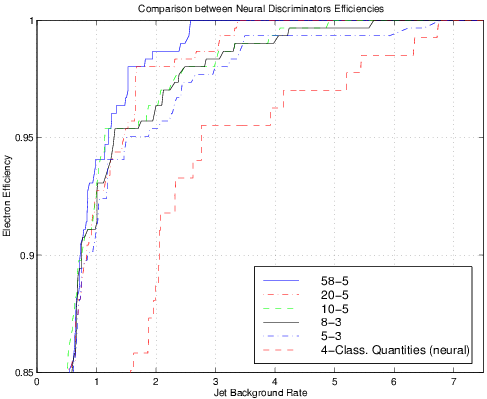
\includegraphics[scale=0.65]{msc/combined}
\end{center}
\caption[Eficiência comparativa entre os melhores discriminadores neuronais
quando o número de entradas varia.]{Eficiência comparativa entre os melhores
discriminadores neuronais quando o número de entradas varia. Os cortes de
dimensionalidade são baseados no critério da relevância, aplicando-se a técnica
do corte direto.}
\label{fig:last-effic}
\end{figure}

\begin{table}
\caption{As variáveis do espaço original de anéis de dimensão 58, após vários
cortes baseados na relevância.} 
\label{tab:left-direct}
\renewcommand{\baselinestretch}{1}
\begin{center}
\small
\begin{tabular}{||c||c||l||l||} \hline
\hhline{|t:=:t:=:t:=:t:=:t|}
Patamar & \# An�is & Calor�metro & An�is Restantes \\
\hhline{|:=::=::=::=:|}

\multirow{4}{30pt}{$0,001$} & \multirow{4}{30pt}{$20$} &
\eng{Presampler} & 1, 2, 4 e 6 \\
\hhline{||~||~||-||-||}
& & 1\eira\ camada e.m. & 7, 8, 9, 10, 11, 12 e 39 \\ 
\hhline{||~||~||-||-||}
& & 2\eira\ camada e.m. & 40, 41, 42, 43, 44, 45 e 46 \\
\hhline{||~||~||-||-||}
& & 1\eira\ camada hadr�nica & 50 e 51 \\
\hhline{|:=::=::=::=:|}

\multirow{4}{30pt}{$0,003$} & \multirow{4}{30pt}{$10$} &
\eng{Presampler} & 1, 2 e 6 \\
\hhline{||~||~||-||-||}
& & 1\eira\ camada e.m. & 7, 8 e 39 \\
\hhline{||~||~||-||-||}
& & 2\eira\ camada e.m. & 40, 41 e 42 \\
\hhline{||~||~||-||-||}
& & 1\eira\ camada hadr�nica & 50 \\
\hhline{|:=::=::=::=:|}

\multirow{3}{30pt}{$0,005$} & \multirow{3}{30pt}{$8$} &
\eng{Presampler} & 1 e 2 \\
\hhline{||~||~||-||-||}
& & 1\eira\ camada e.m. & 7, 8 e 39 \\
\hhline{||~||~||-||-||}
& & 2\eira\ camada e.m. & 40, 41 e 42 \\
\hhline{|:=::=::=::=:|}

\multirow{3}{30pt}{$0,05$} & \multirow{3}{30pt}{$5$} &
\eng{Presampler} & 1 \\
\hhline{||~||~||-||-||}
& & 1\eira\ camada e.m. & 7 e 8 \\
\hhline{||~||~||-||-||}
& & 2\eira\ camada e.m. & 40 e 41 \\

\hhline{|b:=:b:=:b:=:b:=:b|}

\end{tabular}

\normalsize
\renewcommand{\baselinestretch}{1.5}
\end{center}
\end{table}

\typeout{ *************** End of file msc.tex *************** }
